\documentclass{elsart}
\usepackage[dvips]{color,graphics}
\usepackage[pdftex]{graphicx}
\usepackage{lineno}
\linenumbers
%
% macro definitions

%\setcounter{tocdepth}{1} % Show sections
%\setcounter{secnumdepth}{0}


%\setcounter{bottomnumber} {1}
%
%\pagenumbering{arabic}
%
\begin{document}

% -------------------------------------------------
%  title page
% -------------------------------------------------
\begin{frontmatter}
  
\title{The CLAS12 Drift Chamber System}

\author{M.D. Mestayer$^a$ et al.}


% -------------------------------------------------
%abstract
% -------------------------------------------------

\begin{abstract}
The CEBAF Large Acceptance Spectrometer built for the 12~GeV upgrade of Jefferson Lab
(CLAS12) is located in Hall~B and is built around a superconducting toroidal magnet. The six coils
of this toroid divide the detector azimuthally into six sectors.  Each sector contains three multi-layer 
drift chambers for reconstructing the trajectories of charged particles originating from a fixed target.  

Each of the 18 planar chambers has two ``superlayers'' of six layers each, with the wires in the two adjacent
superlayers oriented at $\pm 6^{\circ}$ stereo angle, respectively. Each layer has 112 hexagonal cells
spanning a range from about $5^{\circ}$ to $40^{\circ}$ in polar angle. The six-layer structure provides
redundancy in track segment finding and good tracking efficiency even in the presence of some individual
wire inefficiency.  The design, construction, operation, and calibration methods are described, and estimates
of efficiency and resolution are presented from in-beam measurements.
\end{abstract}



\end{frontmatter}
%\tableofcontents
%\listoffigures
%\listoftables


\section{Forward Tracking System}
\label{overview}

The CLAS12 forward detector is constructed around a toroidal magnet consisting of six 
iron-free superconducting coils.  The particle detection system consists of drift 
chambers to determine charged-particle trajectories, {\v C}erenkov detectors 
for electron/pion separation, scintillation counters for flight-time 
measurements, and calorimeters to identify electrons and high-energy neutral 
particles.  An overview of the CLAS12 subsystems and geometry may be found in the 
CLAS12 Overview paper ~\cite{clas12-overview} in this volume.  A schematic view of the 
torus magnet with drift chambers
attached is shown in Fig.~\ref{chambers-and-torus}.   This assembly is referred to
as the ``forward tracker''. 

The forward tracker can detect charged particles emerging from the target with
momenta greater than 200~MeV/c over a polar angular range from roughly 5$^{\circ}$ to 
40$^{\circ}$.  Because the coils of the torus magnet represent a ``dead area''
in which we cannot detect charged particles, we designed the chamber endplates
and attached electronics to be as thin as possible.  The resulting azimuthal
coverage varied from 50\% of 2$\pi$ at 5$^{\circ}$ to 80\% of 2$\pi$ at 40$^{\circ}$.


%%%%%%%%%%%%%%%%%%%%%% Figure : CLAS 3D Picture %%%%%%%%%%%%%%%%%%%%%%%%%%%%%%%
\begin{figure}[htbp]
\vspace{10cm}
\begin{picture}(50,50)
\put(-10,10)
{\hbox{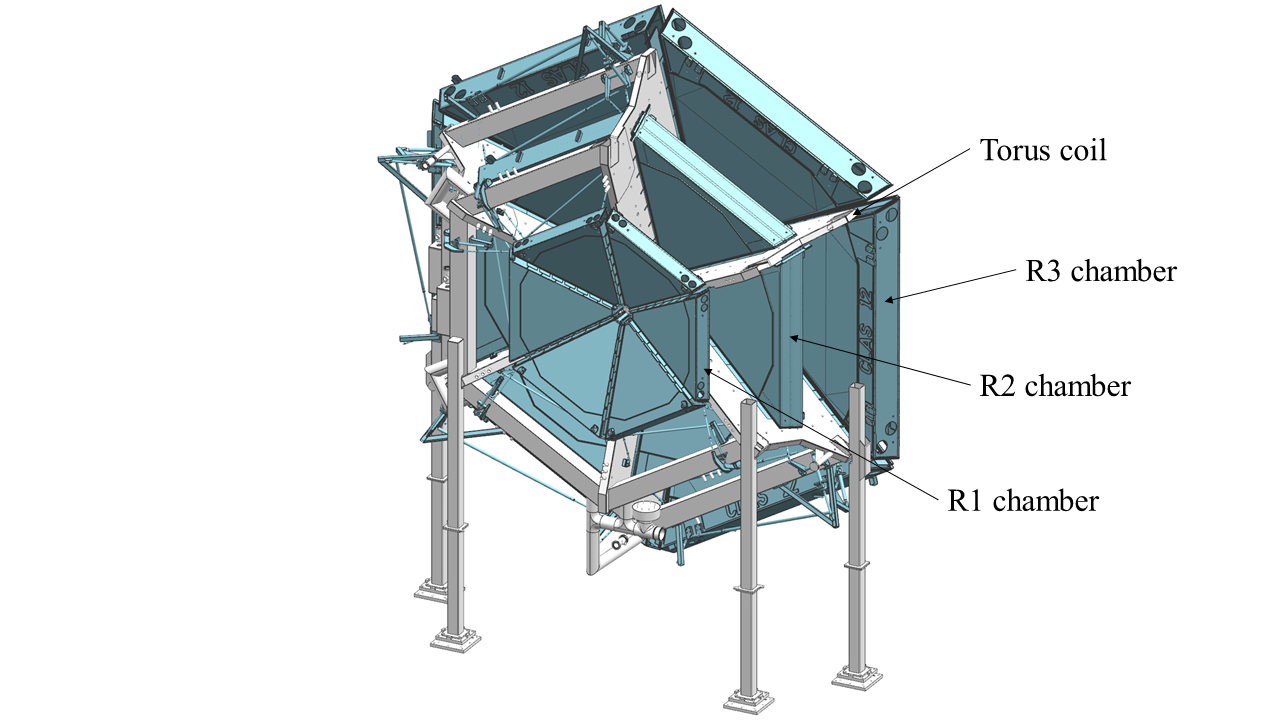
\includegraphics[width=1.\textwidth,natwidth=610,natheight=642]{img/chambers-and-torus.png}}}
\end{picture}
\caption{\small{A sketch of the torus magnet with drift chambers attached.
Note that cable runs and gas lines have been removed for clarity.  The largest
(R3) chambers are approximately equilateral triangular solids with 4 m long sides
and 0.8 m depth.}}
\label{chambers-and-torus}
\end{figure}
%%%%%%%%%%%%%%%%%%%%%%%%%%%%%%%%%%%%%%%%%%%%%%%%%%%%%%%%%%%%%%%%%%%%%%%%%%%


The requirements of the planned physics experiments drove the conceptual design
of the chambers; those requirements and engineering considerations led to 
the final design and construction of the chambers, as discussed in the next section.




















































% -------------------------------------------------
% physics goals -> tech. specs. -> conceptual design
% -------------------------------------------------

\section{Drift Chamber System Conceptual Design}

When the CLAS detector~\cite{clasnim} was upgraded to become the CLAS12 detector, the
drift chambers were re-designed.  We kept many of the design concepts of the original CLAS
chambers~\cite{dcnim}, but made improvements in a number of areas.

\subsection{Physics Requirements for CLAS12 Forward Tracking}

There are several broad areas of physics research that drive the design of the forward tracking system: 
spectroscopic studies of excited baryons, investigations of 
the influence of nuclear matter on propagating quarks, studies of polarized 
and unpolarized quark distributions, and a comprehensive measurement of 
generalized parton distributions (GPDs). 

The cross sections for these processes are small, necessitating high-luminosity 
experiments.  A variety of experiments rely on luminosities of 
10$^{35}$~cm$^{-2}$s$^{-1}$ to achieve the desired statistical accuracy in 
runs of a few months duration.  This is an order of magnitude increase
compared to the previous CLAS detector.  

The new kinematic range available to the CLAS12 experiment is
characterized not only by smaller cross sections, but also by more outgoing 
particles per event, with those particles being emitted at larger momenta
and smaller laboratory angles.  
A final state of a few high-momentum, forward-going particles (the electron as well as one 
or more mesons), combined with a moderate-momentum baryon emitted at large 
angles, is the typical event type that determines the specifications of the 
tracking system. 

To cover as much of the hadronic center-of-mass region as possible, the CLAS12 Forward 
Tracker must provide tracking for charged particles emitted at polar angles 
from 5$^\circ$ to 40$^\circ$.  This is complemented by the angular coverage of
the central tracking system, which covers polar angles from  35$^\circ$ to approximately 125$^\circ$.

In addition to large acceptance, our experimental program requires
small systematic uncertainties.  To measure our electroproduction cross sections
to an accuracy of a few percent, we must know the scattered electron's
momentum to $1\%$ and its angle to 1~mrad.  

We need even better momentum resolution on the scattered
electron (with momentum up to 10~GeV) to be able to identify particles
by missing mass, an important technique in exclusive reaction studies.
We performed tracking simulations assuming perfect knowledge of the drift chamber
location (alignment) and perfect knowledge of the magnetic field, and assuming
that the hit resolution in each of the drift chamber layers was $250~\mu$m.
These calculations are shown in Fig.~\ref{simulated-resolution}, where we
plot the estimated fractional momentum resolution (left axis) vs. momentum
for different incoming angles (right axis) as a function of momentum.

%%%%%%%%%%%%%%%%%%%%%% Figure : generic chamber sketch %%%%%%%%%%%%%%%%%%%%%%
\begin{figure}[htpb]   
\vspace{4.5cm}
\begin{picture}(35,35)
\put(10,-40)
{\hbox{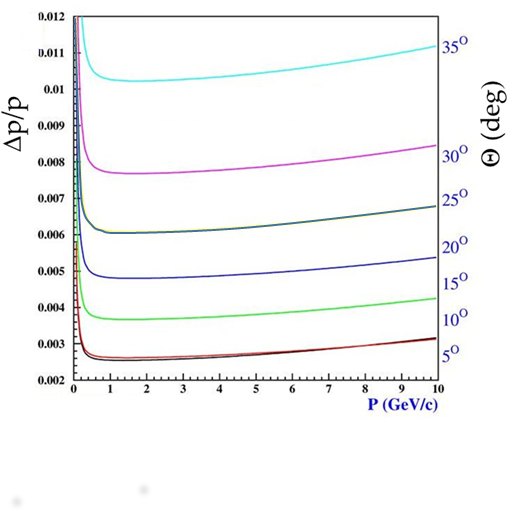
\includegraphics[width=1.5\columnwidth,natwidth=610,natheight=642]{img/simulated-resolution.png}}}
\end{picture}
\caption{\small{Estimated fractional momentum resolution plotted vs. momentum for different
track angles.}}
\label{simulated-resolution}
\end{figure}   
%%%%%%%%%%%%%%%%%%%%%%%%%%%%%%%%%%%%%%%%%%%%%%%%%%%%%%%%%%%%%%%

These simulations led to our goal of $dp/p \approx 0.3\%$ 
for electrons emitted at small angles ($7^{\circ}$) and high momentum (10~GeV).
This requires very good position resolution per hit (on the order of 250~$\mu$m),
very good positional alignment of the chambers ($\approx$50~$\mu$m), and very good knowledge
of $\int \!\!Bdl$ on the order of 0.2\%.  These goals drive our calibration efforts; for more
information see Section~\ref{calibration}.

Table~\ref{fwd-dc-physics-specifications} lists the physics goals for the main CLAS12 program
and the resulting drift chamber design specifications that will allow us to achieve these goals.

%%%%%%%%%%%%%%%%%%%%%%%%%%%%%%%%%%%%%%%%%%%%%%%%%%%%%%%%%%%%%%%%%
\begin{table*}[ht]
\begin{center}
\begin{tabular}{||c|c|c||} \hline \hline
   {\bf Goal}         & {\bf Physics Spec./Goal$^*$} & {\bf Design Specification}\\ \hline
Measure   & $d \theta <$ 1~mrad   & planar chambers \\ 
cross section & $\sin \theta ~d \phi < $1~mrad & $\pm 6^\circ$ stereo angle   \\ 
to 2\% accuracy  & $dp/p < 1\% $ & identical cells (each superlayer)  \\ \hline
Select exclusive reaction; & $^*$$dp/p < 0.3\%$ at 10~GeV   & $250~\mu$m  accuracy per cell\\ 
only one missing particle    &  &    chamber alignment $<100~\mu$m\\  \hline
Small       & Luminosity = $10^{35}$~cm$^{-2}$s$^{-1}$  & six 6-layer superlayers \\ 
cross sections  & high efficiency & $> 95\%$ layer efficiency \\ \hline
large acceptance   & $\delta\phi = 50\%$ at $5^\circ$ & thin endplates\\ \hline
\end{tabular}
\caption{\small{Physics goals and the resulting physics and drift chamber design specifications.}}
\label{fwd-dc-physics-specifications}
\end{center}
\end{table*}
%%%%%%%%%%%%%%%%%%%%%%%%%%%%%%%%%%%%%%%%%%%%%%%%%%%%%%%%%%%%%%%%%

\subsection{Drift Chamber Conceptual Design}

Because the previous CLAS drift chamber system operated 
successfully for 15~years, we re-used many of the design concepts and 
most of the utility infrastructure, including
parts of the gas mixing and handling system, the high voltage 
and low voltage systems, and many of the high voltage and signal cables. 
Refer to our article on the previous CLAS detector~\cite{clasnim} and our article 
on the previous drift chambers themselves~\cite{dcnim} for details.

We kept the same chamber layout as in CLAS:
the forward-tracking system consists of three regions divided into six
sectors as shown in Fig.~\ref{chambers-and-torus}; located just before, inside, 
and just outside the torus field volume, named Regions~1, 2, 
and 3 (and referred to as R1, R2, and R3), respectively.  
Each chamber has its wires arranged in two superlayers (SLs) of
six layers each, with the wires in the two superlayers strung with 
$\pm$6$^\circ$ stereo angles to each other.  The cell structure is 
hexagonal, that is, each sense wire is surrounded by six field wires.  This 
arrangement offers good resolution with very good pattern recognition properties.  

The major difference compared to the previous design is that the 
chambers are located further downstream from the target and thus the drift
cells cover a smaller solid angle than those in the previous CLAS 
chambers, allowing efficient tracking at higher luminosities because the 
accidental occupancy from particles not associated with the event is smaller.  

\subsection{Design Features}

Table~\ref{fwd-dc-design-parms} lists the main design parameters for each 
region of the CLAS12 drift chambers.  For the purposes of simulating 
track resolutions, we assumed that the position resolution of the individual 
drift cells would be 250~$\mu$m.  The material budget for multiple scattering
consists of about 0.02 radiation lengths before the R1 chambers due to an assumed 5~cm LH$_2$
target, the gas and low-mass mirrors in the Cherenkov counter, and the remainder of air.
The total material in the R1, R2 and R3 chambers (each filled with a 90/10 mixture
of argon/CO$_2$) and the intervening air also amounts to $\sim$0.02 radiation lengths.

%%%%%%%%%%%%%%%%%%%%%%%%%%%%%%%%%%%%%%%%%%%%%%%%%%%%%%%%%%%%%%%
\begin{table*}[hbt]
\begin{center}
\begin{tabular}{||c|c|c|c||} \hline \hline
            &{\bf Region 1}&{\bf Region 2}&{\bf Region 3}\\ \hline
Distance from target & 2.3~m    & 3.5~m        & 4.9~m    \\ \hline
Num. of superlayers  & 2        & 2            & 2        \\ \hline
Layers/superlayer    & 6        & 6            & 6        \\ \hline
Wires/layer          & 112      & 112          & 112      \\ \hline
Cell radius (each SL) & 0.78, 0.81~cm  & 1.14, 1.32~cm      & 1.87, 1.96~cm  \\ \hline
Active time window   & 150~ns   & 325 - 1000~ns & 750~ns   \\ \hline
\end{tabular}
\caption{\small{Design parameters for the CLAS12 drift chambers.}}
\label{fwd-dc-design-parms}
\end{center}
\end{table*}
%%%%%%%%%%%%%%%%%%%%%%%%%%%%%%%%%%%%%%%%%%%%%%%%%%%%%%%%%%%%%%

%%%%%%%%%%%%%%%%%%%%%% Figure : generic chamber sketch %%%%%%%%%%%%%%%%%%%%%%
\begin{figure}[htpb]   
\vspace{3cm}
\begin{picture}(35,35)
\put(15,0)
{\hbox{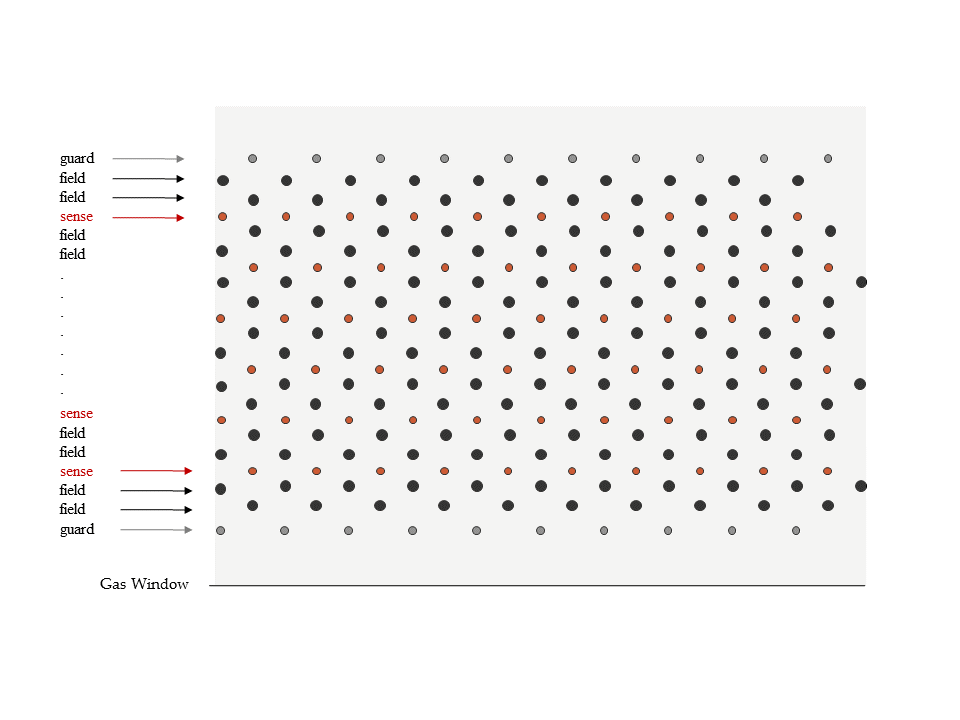
\includegraphics[width=0.9\columnwidth,natwidth=610,natheight=642]{img/superlayout.png}}}
\end{picture}
\caption{\small{Wire layout for one superlayer; the view is a cut perpendicular to the wire direction.}}
\label{superlayout}
\end{figure}   
%%%%%%%%%%%%%%%%%%%%%%%%%%%%%%%%%%%%%%%%%%%%%%%%%%%%%%%%%%%%%%%

\subsubsection{Design Elements in Common with the Previous CLAS Chambers}

The CLAS12 drift chambers share some design characteristics with the previous CLAS chambers:
\begin{itemize}
\item {\bf Wire Layout}
\begin{itemize}
\item ``brick-wall'' wire layout resulting in individual hexagonally shaped
drift cells in a plane perpendicular to the wire direction;
\item sense wire layers are grouped into two ``superlayers'' of 6 layers each;
\item the ``endplates'' on the two sides of the chamber are tilted 
at $\sim$60$^\circ$ with respect to each other.
\end{itemize}
\item {\bf Chamber Body Design}
\begin{itemize}
\item to maximize the active volume of the chamber, the ``dead areas'', e.g.
the endplates and electronics boards, are kept as thin as possible;
\item because of the possibility of large eddy currents and resultant
force on the endplates in case of the quench of our torus magnet, we again
use non-conducting Stesalit 4411W endplates for our R2 chambers; (``Stesalit'' is 
a trademark of STESALIT AG for a disordered epoxy-fiberglass composite product.  See
Ref.~\cite{dcnim} on the previous CLAS drift chambers for more information.);
\end{itemize}
\item {\bf Gas Choice:} 90:10 argon:CO$_2$ mixture.  We operate at a gas gain of 
about $5 \times 10^4$.
\end{itemize}

Figure~\ref{superlayout} is a schematic of the cell layout for a single superlayer.
The wires are arranged in a ``brick wall'' pattern with one layer of guard wires,
two layers of field wires, one layer of sense wires, another two layers of field
wires, and so on, for a total of 2 guard wire layers, 14 field wire layers and
6 sense wire layers.  The result is an hexagonal cell layout with each sense wire
surrounded by 6 field wires.

\subsubsection{Design Improvements Compared to the Previous CLAS Chambers}

To improve the chambers' performance we made some important changes to the design:
\begin{itemize}
\item {\bf Mechanical Design}
\begin{itemize}
\item all chambers have the same, roughly equilateral triangular, shape;
\item the previous CLAS chambers were interconnected to each other (R1) or 
connected directly to the torus (R2).  In the present chambers all of the wire tension
is borne by the endplates and thus they can be independently mounted.
The key to this improvement is the use of  
ultra-stiff endplate assemblies that obtain their stiffness 
by a flanged design;
\item all chambers are independent and self-supporting, allowing easy
maintenance and repair.  The chambers are attached to the torus cryostat using 6 independent
rods arranged in a ``ball-and-socket'' linkage system, enabling the chambers to
be moved out to their maintenance position and back to the operating 
position by turning one precision turn-buckle assembly.
\end{itemize}
\item {\bf Cell Design and Wire Layout}
\begin{itemize}  
\item For the previous CLAS detector, the $\phi$ resolution times $\sin \theta$ was about two 
times larger than the $\theta$ resolution.  To have more equal resolution in 
the two angles, we doubled our stereo angle from 0 and 6$^\circ$ to 
$\pm$6$^\circ$;
\item all chambers are planar, with the first superlayer (of 6 layers)
tilted at a 6$^\circ$ stereo angle, and the second superlayer at a -6$^\circ$ stereo angle;
\item all wires within one superlayer are parallel to each other, thus
every cell in one superlayer is identical, making it easier to model
and fit the distance-to-time response.
\end{itemize}
\item {\bf Wire Choice}
\begin{itemize}
\item all chambers are strung with 30-$\mu$m gold-plated tungsten wire,
considerably tougher and easier to handle than our previous choice 
of 20-$\mu$m wire;
\item the choice of the cathode (``field'') wire is 80-$\mu$m
gold-plated copper-beryllium, tougher and with better surface properties than our previous
choice of 140-$\mu$m gold-plated aluminum wire;
\item  Our choice of guard wire is 140-$\mu$m diameter, gold-plated
copper-beryllium.  These wires were strong enough that we pre-tensioned 
the chambers using only the guard wires; a simplification in the process.
\end{itemize}
\end{itemize}

Table~\ref{fwd-dc-design-features} lists the advantages and disadvantages
of the various design features.

%%%%%%%%%%%%%%%%%%%%%%%%%%%%%%%%%%%%%%%%%%%%%%%%%%%%%%%%%%%%%%%%
\begin{table*}[ht]
 \begin{center}
  \begin{tabular} {||c|c|c||} \hline \hline
 {\bf Design Feature}       &{\bf Advantages} &{\bf Disadvantages}\\ \hline
``All-wire design'' & Little cathode emission & \\ \hline
Small Cells & Robust track-finding  & Many wires to string \\ \hline
Hexagonal Cells & Minimum number of wires  & Angle-dependence of time to distance  \\ \hline
30~$\mu$m diameter sense wire & Resistant to wire breakage & Higher operating voltage \\ \hline
80~$\mu$m diameter field wire & Lower total wire tension & Higher fields on cathode wires \\ \hline
Opposite voltage  & Identical fields & More HV \\
for sense and field & for all layers & channels required \\ \hline
Self-supporting design & Easier maintenance & 1 - 2~mm bowing of endplates \\ \hline
\end{tabular}
\caption{\small{Design features of the CLAS12 drift chambers.}}
\label{fwd-dc-design-features}
\end{center}
\end{table*}
%%%%%%%%%%%%%%%%%%%%%%%%%%%%%%%%%%%%%%%%%%%%%%%%%%%%%%%%%%%%%%%%

\subsubsection{Wire Diameter}

One of the most significant design changes was the decision 
to use 30-$\mu$m diameter sense wire rather than the previously used 
20-$\mu$m wire. This should make the chambers more resistant to wire 
breakage.  The larger radius of the sense wires means that higher 
voltages will be required to achieve the same gas gain, see
Section~\ref{determine-operating-parameters} for more details.
Prototypes were built to study possible negative side-effects of the 
higher voltage operation, such as leakage currents on the circuit boards 
and/or higher rates of cathode emission from the field wire surfaces.
No such effects were seen.
We discuss the wire choice in more detail in Section~\ref{construction}.



 


% -------------------------------------------------
% design: ``box'' design, feedthoughs and pins, wire choice, gas choice, mechanical connections
% -------------------------------------------------

\section{Chamber Construction}
\label{construction}

\subsection{Construction Overview}

The three chamber types (called ``regions'', with ``Region 1'' abbreviated as 
``R1'', etc.)  share the same basic design elements simply
scaled up in size by a factor of 1.5 for R2 relative to R1 and a factor
of 2 between R3 and R1. Each chamber is a solid trapezoid in shape, with  
a pair of wire-supporting endplates that bear both the load of the 
wire tensions and the weight of all associated hardware. A representative 
chamber is shown in Fig.~\ref{chamber-exploded}, with the component parts indicated.
This particular drawing is of a R1 chamber, but all chambers have the
same basic parts.

%%%%%%%%%%%%%%%%%%%%%% Figure : generic chamber sketch %%%%%%%%%%%%%%%%%%%%%%
\begin{figure}[htpb]   
\vspace{10cm}
\begin{picture}(35,35)
\put(-70,0)
{\hbox{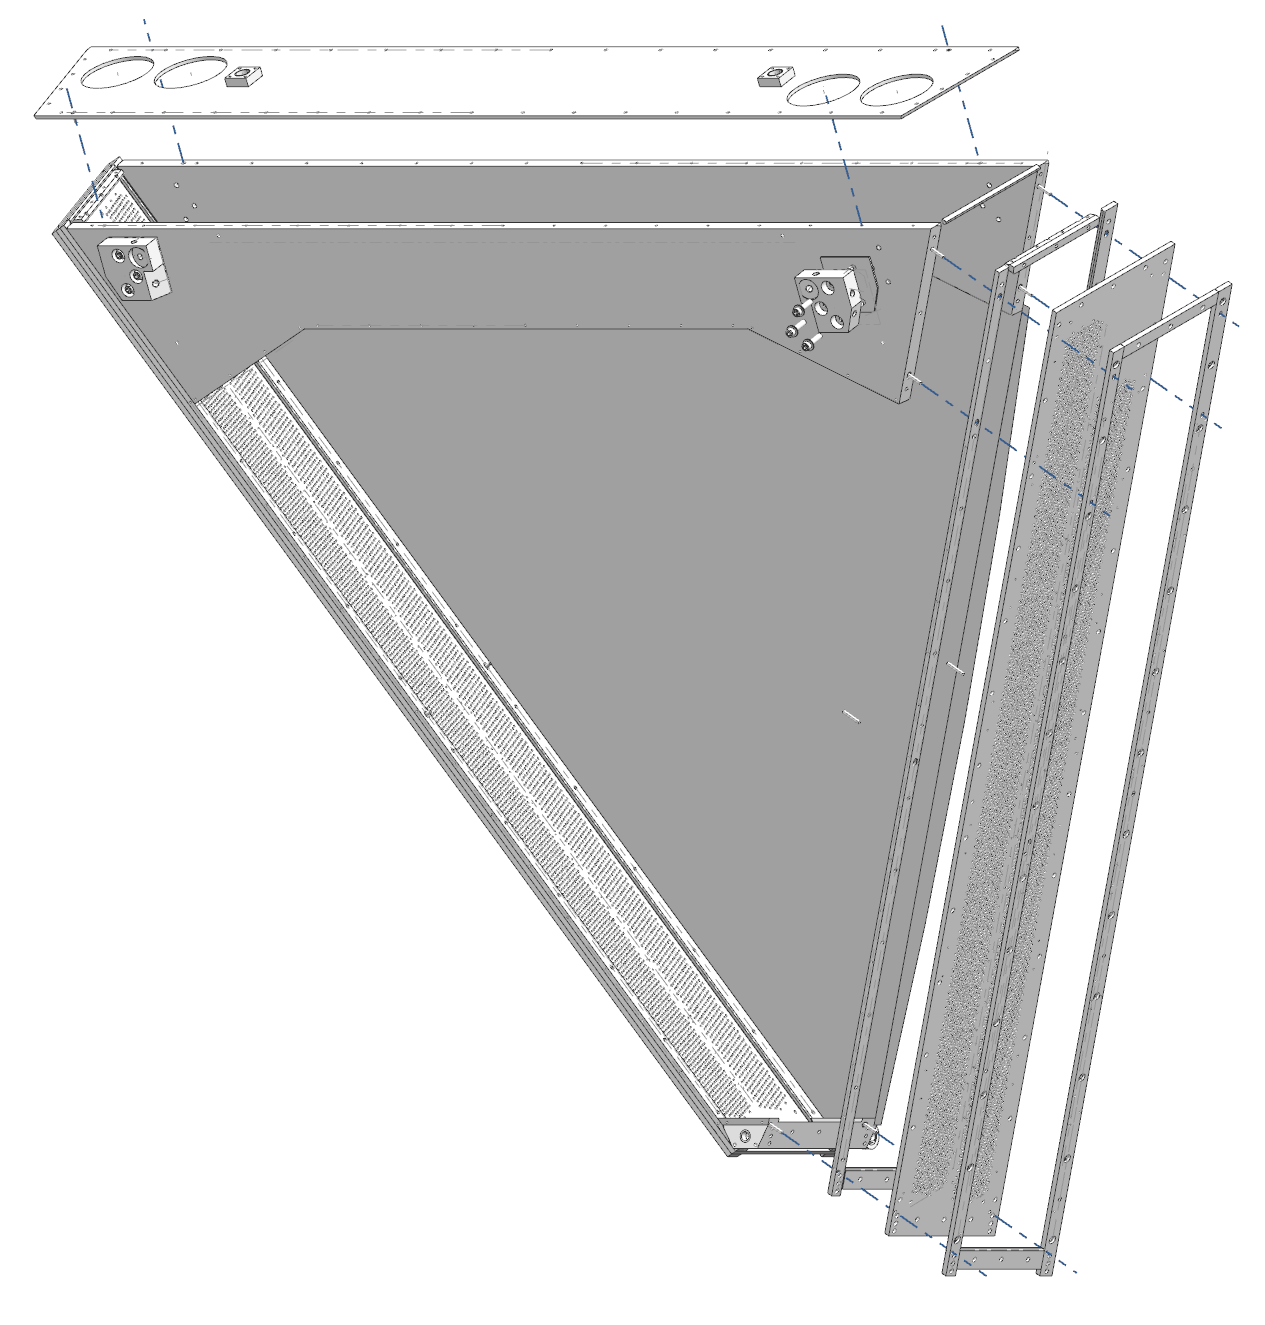
\includegraphics[width=0.9\columnwidth,natwidth=610,natheight=642]{img/chamber-exploded.png}}}
\end{picture}
\caption{\small{Assembly of a typical drift-chamber
(here a R1 sector) highlighting the common component parts.}}
\label{chamber-exploded}
\end{figure}   
%%%%%%%%%%%%%%%%%%%%%%%%%%%%%%%%%%%%%%%%%%%%%%%%%%%%%%%%%%%%%%%

The chamber bodies were constructed from accurately machined plates
(2 endplates, a ``nose-plate'' and a ``back-plate'').
The endplates themselves were an assembly of a main plate with precision-drilled
holes to which we bolted and glued stiffener bars.  In the case of
R1 the main plate was aluminum and the stiffener bars were stainless steel;
for R2 the main plates were non-conducting Stesalit material and the bars stainless steel, and for R3
the main plates were themselves an assembly of two thin steel plates with a foam interior.
No additional stiffener bars were used for R3.

At the radially outward end of each chamber, a thick ``back-plate'' was 
employed to maintain the relative 
alignment of the endplates, to stiffen the chamber against bending moments, 
and to provide a place to attach gas seals and fittings. At the radially inward 
end of each chamber, the endplates were connected together via a small joining 
piece called the ``nose-plate''.  The hardware fabrication and placement 
was of critical importance to the dimensional accuracy of the chambers.

We used many of the same construction materials and procedures as we did
in the previous CLAS chambers.  Please see the previous NIM article \cite{dcnim} 
for these details.  For the reader's convenience, we repeat some of the descriptions
in this article.

\subsection{Construction Materials}
\label{materials}

To ensure a long working life for the chambers, care was taken to 
specify that all materials in contact with the gas volume were clean and ``chamber 
safe'' as defined in Ref.~\cite{kadyk}.  As previously, all construction was carried out in 
Class-10000 or better clean rooms.

The drift-chamber bodies were made primarily of aluminum (R1), Stesalit (an epoxy-fiberglass composite) (R2),
or steel-clad structural foam (R3).  See Section~\ref{region2} for more discussion
of the properties of Stesalit.  The aluminum and steel parts were 
manufactured with machine oils and, as before, were subsequently cleaned with  
Micro-laboratory detergent from the Cole-Parmer Instrument Company.  The 
Stesalit endplates were machined without any lubricating oils.  Immediately 
prior to chamber assembly all parts were cleaned with detergent, then rinsed with
deionized water and alcohol.  The various wire attachment parts, feedthroughs and
crimp pins, were cleaned in an ultrasonic bath 
with detergent and then rinsed in a second ultrasonic bath with deionized water.

It is important to avoid any outgassing into the chamber.  As in the construction
of the previous CLAS chambers, we used Shell Epon resin 826 mixed with Versamid 140, and 
Scotchweld varieties 210 and 2216 for chamber assembly and gluing of feedthroughs.  These mixtures have been 
studied extensively and found not to outgas significantly~\cite{nasa}.

As before, the on-chamber gas tubing is mainly stainless steel, with some
nylon tubing used in the gas manifolds.  Special care was taken during
all steps of construction and testing to ensure that no oils or
silicones contacted any of the chamber materials.

\subsection{Chamber Body Construction}

The construction of the chamber bodies consisted of 3 main stages:
\begin{itemize}
\item receipt, inspection, and cleaning of parts,
\item assembly of the main drilled plate and stiffener bars into a complete endplate,
followed by insertion and gluing of the feedthroughs into the pre-drilled holes 
in the main plate, and 
\item over-all assembly of the endplates and nose- and back-plates to make
a chamber ``box''.
\end{itemize}

\subsubsection{Inspection and Cleaning}

After a visual inspection, we first cleaned the endplates and structural 
frame using a low residue laboratory degreasing solution and water rinse.
We then performed a final cleaning using an ultrasonic bath of a laboratory-grade detergent solution.  
After two hours we rinsed with de-ionized water and then sprayed 
with methanol to aid drying.
We cleaned the feedthroughs and other small parts with a similar procedure.
In addition, the injection-molded parts were specified to be free of silicon 
mold releases.
 
\subsubsection{Endplate and Chamber Body Assembly}

We assembled the endplates on a table in the cleanroom.  The various parts,
the pre-drilled main plate and the various stiffener bars, were pinned
and glued into place.  Once the endplate assembly was finished,
we inserted and glued feedthroughs into each hole.  We took special care 
to use the minimal amount of glue required to provide a solid gas 
seal in order to prevent glue contamination inside the detector. 

The feedthroughs are an assembly of a flared metal tube, a `` trumpet'', fitted into an injection-molded 
plastic feedthrough.  The metal trumpets were produced on a screw machine, and 
delivered to the injection molding factory.
As with the original CLAS chambers we specified the use of
``Noryl'' plastic reinforced with glass beads to make it stiffer.
It is important to note that the surface conductivity
of this glass-bead loaded composite is little affected by room humidities
as high as 60\%, in contrast to similar plastic strengthened
with microscopic glass strands which performed poorly in high-voltage stand-off
tests in humid conditions.  

Because our chamber endplates are not parallel, but oriented at
$\approx 60^{\circ}$ with respect to each other, the wire position is determined
by the feedthrough's trumpet's concentricity and placement and not by
the concentricity or inner radius of the crimp pin; see Figures~\ref{wire-attachment} and ~\ref{dc-corner}.

This allowed us to design the crimp pin to maximize crimp reliability
and ease of use by using soft copper with a large enough inner diameter
to be used for stringing all types of wire: sense, field and guard.
Using a thick-walled copper pin ensured a good crimp through a range of gap settings~\cite{sbc}.
Having a single type of crimper required fewer re-calibrations; the soft
copper made more secure crimps and the larger inner radius made
stringing easier.

 A schematic of the wire attachment schema is shown in
Fig.~\ref{wire-attachment}.  At this stage of endplate construction, the
feedthroughs (part ``2'' in Fig.~\ref{wire-attachment}) were glued into place.
Later, during the wire stringing phase, described in Section~\ref{stringing},
the crimp pins (part ``3'') were fitted into the feedthrough and crimped to
hold the wire.  

%%%%%%%%%%%%%%%%%%%%%% Figure : generic chamber sketch %%%%%%%%%%%%%%%%%%%%%%
\begin{figure}[htpb]   
\vspace{10cm}
\begin{picture}(35,35)
\put(10,0)
{\hbox{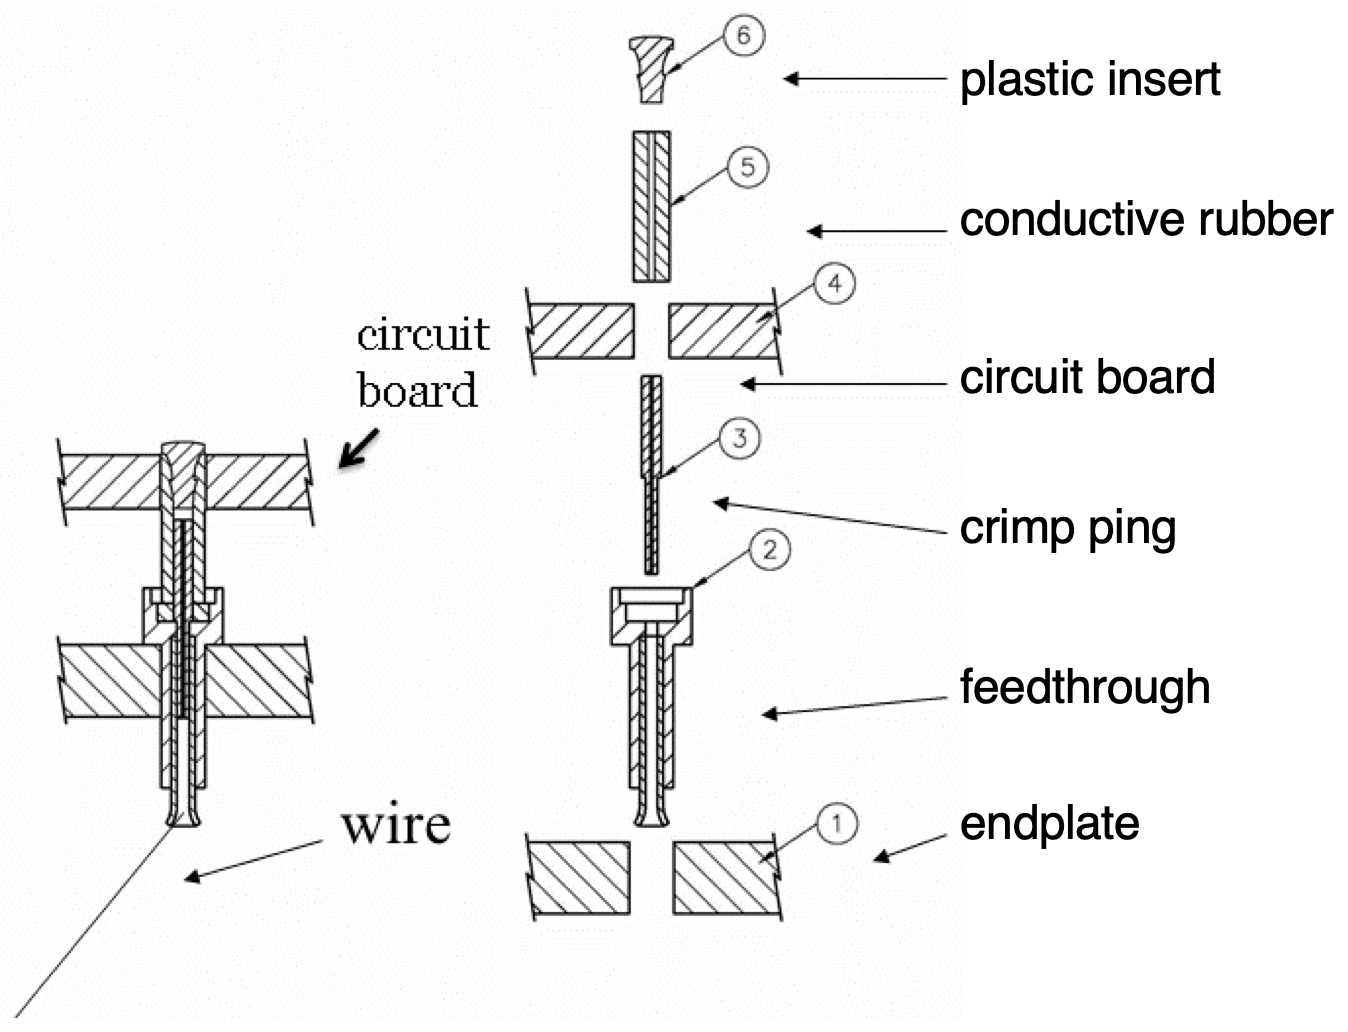
\includegraphics[width=0.9\columnwidth,natwidth=610,natheight=642]{img/wire-attachment.png}}}
\end{picture}
\caption{\small{The collection of all parts used to physically attach a wire end
to a chamber endplate and to provide an electrical connection to a chamber-mounted circuit board.}}
\label{wire-attachment}
\end{figure}   
%%%%%%%%%%%%%%%%%%%%%%%%%%%%%%%%%%%%%%%%%%%%%%%%%%%%%%%%%%%%%%%

Once the endplates were complete with feedthroughs in place, 
we assembled the chamber box from the
endplates, nose-plate, and back-plate using a variety of special-purpose
fixtures.  With the box held in its final configuration, the parts were bolted
and glued into place using the special glues mentioned in Section~\ref{materials}.
We used precision pinning extensively to achieve high dimensional accuracy.

\subsection{Wire Choice}

Our ``thin endplate'' design required minimizing wire tensions and
thus the diameter of the wire.  The real key to reducing wire tension is to
make the field wires (which are much larger than the sense wires) as 
thin as possible and to make them out of low-density metal.  

In general, designers have chosen very small diameter sense wires because they
require lower operating voltages.
The sense wire choice for all of our chambers, supplied by the Luma
Sweden Company, is 30~$\mu$m diameter gold-plated tungsten.  
The previous CLAS drift chambers used 20~$\mu$m diameter wire for the
sense wires.  We decided to use the thicker 30~$\mu$m wire because it is 
significantly tougher, making it easier to handle without
accidental kinking and less likely to break.
As before, Tungsten was chosen because of its durability, 
and we specified gold-plating because it is chemically inert.  

We chose 80~$\mu$m gold-plated Cu-Be wire for our field wire and
140~$\mu$m gold-plated Cu-Be wire for our guard wires; both supplied
by Little Falls Alloys. Cu-Be wire is very tough, is easily plated, and resists
``flaking'' of the gold plating. 
As mentioned, minimizing the field wire diameter is important because it means that they 
could be strung at lower tension than a thicker wire for the same gravitational sag.  
This minimizes the forces on the endplates that we wanted to keep as 
thin as possible to maximize the solid-angle of the sensitive area of
the chambers.

The 80~$\mu$m diameter was chosen because it is the smallest diameter
that will not initiate cathode emission at the surface.
We designed for a gas gain of a few times 
10$^4$; see Section~\ref{operating-voltage} for further discussion of this. 
Under this condition, the electric field at the surface of the sense 
wires is $\approx$200~kV/cm and at the field wire
surface is less than 50~kV/cm, preventing 
conditions that cause unwanted cathode emissions and a noisy chamber.  

We note that our choice violated the ``20~kV/cm rule'', the conventional wisdom that
a surface field greater than 20~kV/cm on the cathode wire would lead to 
a noisy chamber. Our own studies showed that there was no cathode emission below
50~kV/cm from any wire with good surface finish~\cite{cathode-emission} .  Each batch
of wire was evaluated with our test device~\cite{patent} to ensure that at operating field 
values there was no emission.  

\subsubsection{Wire Tensions}

A basic principle of our drift chamber design is that each drift cell is a perfect hexagon
in cross-section.
We used this geometrical constraint to determine the hole placement in the endplates.
This design procedure assumed that wires are straight lines.  Of course, real wires
sag across the wire span due to gravity.  To keep our perfect hexagonally shaped cells,
we tensioned our three types of wires (sense, field, and guard) such that they
sagged equally under their gravitational loads.

Our 30~$\mu$m tungsten sense wires, 80~$\mu$m Cu-Be field wires, and 140~$\mu$m Cu-Be guard
wires had linear densities of 0.014, 0.042, and 0.129~g/m, respectively.  To sag equally
under gravity, they were strung at 20, 62, and 190~g of tension, respectively.
In each chamber there were 12 rows of 112 sense wires, 28 rows of 112 field wires,
and 4 rows of 112 guard wires for a total wire tension of 306~kg.
This caused some bowing of our thin endplates. This bowing and the sagging
of the wires themselves is discussed in the Section~\ref{geom_distortions} on geometrical distortions.

\subsection{Chamber Wire Stringing}
\label{stringing}


Because all of the chambers have the same shape, differing only in
size and some materials, we strung them all using the same basic method.
They were gravity-strung using a similar methodology to that 
used when stringing the previous CLAS drift chambers.  The detector box 
assembly was first mounted to a stringing fixture using the same
``ball and socket'' linkage system that was later used to attach the
chambers to the torus magnet.  

%Fig.~\ref{stringing} is a photograph of two
%of the R3 chambers in the cleanroom, mounted to their fixtures. 
%%%%%%%%%%%%%%%%%%%%%% Figure : generic chamber sketch %%%%%%%%%%%%%%%%%%%%%%
%\begin{figure}[htpb]   
%\vspace{10cm}
%\begin{picture}(35,35)
%$\put(-70,0)
%{\hbox{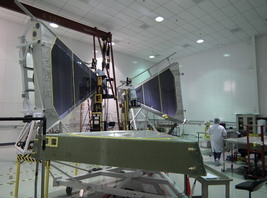
\includegraphics[width=0.9\columnwidth,natwidth=610,natheight=642]{img/stringing.jpg}}}
%\end{picture}
%\caption{\small{Two chambers in the cleanroom ready for stringing.}}
%\label{stringing}
%\end{figure}   
%%%%%%%%%%%%%%%%%%%%%%%%%%%%%%%%%%%%%%%%%%%%%%%%%%%%%%%%%%%%%%%

Under full wire tension, the endplates bow inward as much as 2~mm 
(see Section~\ref{geom_distortions} for a discussion of this issue).
Because of this bowing, it is necessary to pre-tension the chamber
so that the endplates are bowed into their final state at the 
beginning of the stringing process.

We pre-tensioned the chambers by over-tensioning the 140 $\mu$m guard
wires such that the total wire tension load was equal to the final, 
fully strung load.  The over-tensioning was done using an adjustable
spring attached to each guard wire. 
We then strung the field wires, starting at one end of the chamber.
After stringing a ``column'' of 14 field wires, we reduced the
tension on the associated guard wire to its nominal value, and crimped
that guard wire.  In this way, the total wire tension on the endplate
(and its bowing) remained approximately constant through the stringing process.

We strung all chambers with 
the wires running vertically.  The links were adjusted to place the 
feedthroughs in the upper plate vertically above the ``partner''
feedthroughs in the lower plate, which allowed gravity stringing.

The stringing technique began at the top endplate.  The technician attached a 
small steel needle to the wire using a plastic tube with inner diameter only
slightly larger than the radius of the needle.  By inserting both the wire and
needle into the plastic tube, a friction joint was achieved.  
The wire with needle attached was then threaded through the feedthrough in 
the upper endplate.  The wire was then despooled and gravity acted to bring the 
wire close to the feedthrough in the lower endplate.  A small magnet was 
used to pull the needle and wire through the lower feedthrough.  The upper wire
was then cut from the spool and a crimp pin was attached, crimped and seated into
its feedthrough.  After the wire was attached at the upper end, the lower 
crimp pin was slid over the wire and seated into its feedthrough.  Then 
weights were attached to the wire to set the 
proper tension, and the lower crimp pin was crimped, completing the process.

At the beginning of each shift, wires that had been strung on the previous day
were tested in two ways:
\begin{itemize}
\item a continuity test checked that the wire made a good electrical contact
from one feedthough to its partner on the other endplate, and
\item a tension measurement was performed using an ``oscillating wire'' technique.
A static magnetic field was established using large Helmholtz coils.  A sine
wave electric current was established on the wire being tested using a frequency-controlled 
AC power supply.  The AC current could be varied in frequency.  For a 
few-second interval, the Lorentz force on the wire caused it to vibrate and
then during a few-second ``voltage-off'' period, the resulting induced voltage
was read out on an oscilloscope.  In this way, we determined the resonant frequency
of the wire. 
\item if this frequency agreed within limits with a pre-calculated
table of nominal frequency, the wire passed the frequency test.  The tension limits for
the longest wires (length greater than 3m) was $\pm~15\%$, while for the shortest wires
(~ 30 cm) the tension limits were $+50\%$ and $-25\%$.
\end{itemize}
Wires that failed either test were removed and re-strung.

Wires that wrapped around each other while being threaded through the chamber 
were a major contribution to stringing inefficiency. To avoid the wrapping
problem, a machine was built to spool the wire through the chambers quickly and smoothly.
As mentioned earlier, another important development was the design of a crimp pin 
that accepted both the tungsten and copper-beryllium wire types.    This 
eliminated the need to use separate crimping tools, each requiring frequent 
calibrations.  
As a result, the average time to string a wire was less than 4 minutes.

After all wires were strung,
a small amount of glue was applied to the glue well
in the feedthrough to firmly fix the crimp pin in place.  After this ``potting''
operation was done, the chambers were taken off of the stringing fixture and
placed on stands on the floor for final continuity checks.

\subsection{Region One Construction (Special Considerations)}

The R1 chambers were designed and constructed through a collaboration 
of Idaho State University and Jefferson Laboratory.  These 
chambers are located about 2~m from the target, 
before particles enter the magnetic field of the torus,
and are thus key to good angular resolution. 

As is seen from the generic assembly sketch of a chamber (see Fig.~\ref{chambers-and-torus}),
the R1 chambers have a similar shape to the R2 and R3 chambers, differing in
scale and in some material choices.
Most notably, the endplates are constructed of aluminum with stainless
steel stiffener bars.

The main challenges in the R1 construction and design came about because
of the small wire spacing (8~mm between the sense and field wires).  This
increased the electrostatic attraction of neighboring wires if they were
not perfectly and symmetrically placed, and it also made the physical act
of stringing the wires more difficult.

Wires with opposite voltage are electrostatically attracted.  If perfectly
placed in a symmetric array the forces would cancel each other. 
However, the sense wires might be slightly misplaced and so they would feel
a force which, if the tension were below a critical value, would increase
and pull them further out, further increasing the force, and so on until 
the wire begins to oscillate and then spark.  For our electric field configuration
this critical tension was about 3~g, substantially below our nominal
tension of 20~g.



\subsection{Region Two Construction (Special Considerations)}

\hskip 0.15 in 
The R2 chambers, which were designed and constructed by Old Dominion University 
in collaboration with Jefferson Laboratory, are the middle of the three  
drift-chamber packages.  They track all charged particles in the magnetic field 
of the torus near the point of maximum sagitta.  The six identical R2 sectors 
are approximately equilateral triangular boxes with 3 m sides. 
They are located at a radius of $\approx$3~m from the nominal target location.  
  
The R2 chambers were designed with ultra-thin endplates which were thin enough
to be wholly within the ``shadow'' cast by the torus cryostat; in other words,
the full length of the wires is in the active fiducial volume of CLAS12. 
All chamber support hardware and electronics had to fit 
entirely within this shadow region.


Fig.~\ref{dc-corner} shows a slice through a chamber endplate (R2 in this case)
showing some of the wire positioning hardware and attachment of the electronics 
boards.
%%%%%%%%%%%%%%%%%%%%%% Figure : DC Sector Schematic %%%%%%%%%%%%%%%%%%%%%%
\begin{figure}[htpb]   
\vspace{8cm}Schematic cross-sectional view of the R2 endplate showing
wire-positioning hardware.
\special{psfile=img/r2_inserts.eps hscale=70 vscale=70 hoffset=0 voffset=50}  
\caption{\small{}}
\label{dc-corner}
\end{figure}   
%%%%%%%%%%%%%%%%%%%%%%%%%%%%%%%%%%%%%%%%%%%%%%%%%%%%%%%%%%%%%%%%%%%%%%%%%%


The R2 chambers have to operate 
in a magnetic field up to 2~T, and the chambers have to withstand any rapid 
changes in magnetic field, such as what might occur due to a magnet quench.
The R2 endplates are constructed from 2-cm thick Stesalit 4411W, a disordered 
epoxy-fiberglass composite commonly used in wire-chamber construction
\cite{stesalit}, and known not to cause aging problems~\cite{stesalitaging}.  
Using a nonconducting material eliminates any possible forces on the endplate 
due to eddy currents produced during a magnetic-field quench.  

The ``stesalit'' composite is not very stiff and, if not reinforced, would
bend excessively under the load of wire tension.  So, as in the case of
the R1 chambers, the R2 endplates were a composite structure with
stainless steel stifferners.  Fig.~\ref{dcr2-endplate} shows an assembly drawing of an R2 endplate.

%%%%%%%%%%%%%%%%%%%%%% Figure : generic chamber sketch %%%%%%%%%%%%%%%%%%%%%%
\begin{figure}[htpb]   
\vspace{10cm}
\begin{picture}(35,35)
\put(10,-10)
{\hbox{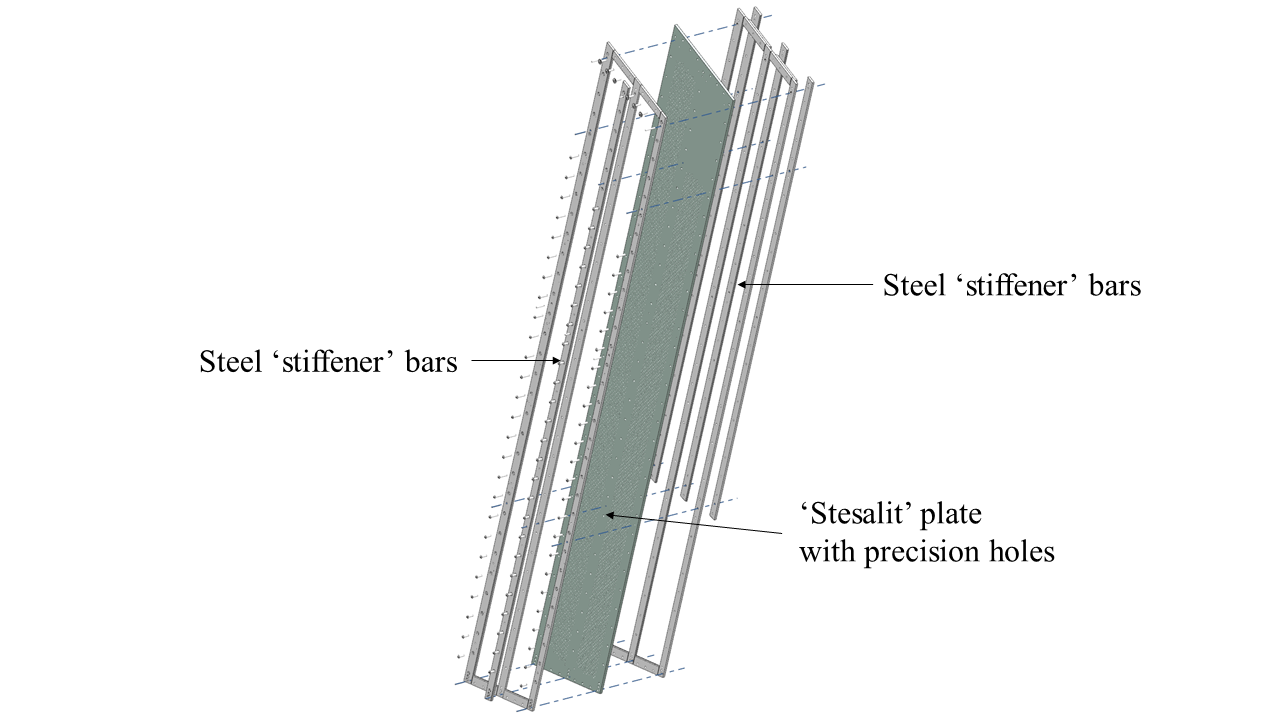
\includegraphics[width=0.5\columnwidth,natwidth=610,natheight=642]{img/dcr2-endplate.png}}}
\end{picture}
\caption{\small{A R2 endplate assembly.}}
\label{dcr2-endplate}
\end{figure}   
%%%%%%%%%%%%%%%%%%%%%%%%%%%%%%%%%%%%%%%%%%%%%%%%%%%%%%%%%%%%%%%%%%%%%%%%%%

It also allows 
the trumpets that position the wires to be essentially flush with the endplates, 
rather than having to insulate the trumpets from the conducting endplates as in 
the other two Regions (see Fig.~\ref{dc-corner}).  This reduced the thickness of 
the inactive region by 1 to 2~cm.




 



\subsection{Region Three Construction}

\hskip 0.15 in
The R3 chambers were designed and constructed at Jefferson Laboratory.  
They had the same general shape as the other chambers but were larger,
4 m on a side so the wires were as long as 4 m.
To reduce the gravitational sag of these very long wires we
strung them at 40 grams, twice the nominal tension of 20 grams.

%%%%%%%%%%%%%%%%%%% Figure : Region Three Cross Section %%%%%%%%%%%%%%%%%%
\begin{figure}[htpb]
\vspace{7.9cm}
\caption{\small{Assembly drawing of a R3 chambers showing the component
parts and highlighting the Carbon fiber tubes at the entrance face and
the carbon-foam composite plate at the exit, which supported the endplates
agains the wire tension.}}
\label{r3_cut}
\end{figure}
%%%%%%%%%%%%%%%%%%%%%%%%%%%%%%%%%%%%%%%%%%%%%%%%%%%%%%%%%%%%%%%%%%%%%%%%%%%

Because these are the final tracking chambers, multiple scattering
at the chamber entrance is not as important as multiple scattering that
occurs at a R1 or a R2 chamber, for example.  This allowed us to 
build a chamber in which the endplates were not supported only on
their ends.  At the entrance face we included 7 thin-walled Carbon
fiber tubes to span the gap and hold the endplates apart.  At the
exit face the endplates were coupled to a triangular carbon-foam-carbon
composite plate which similarly supported the wire tension.









% -------------------------------------------------
% construction: box assembly, stringing, board installation & cabling, gas manifolds
% -------------------------------------------------

\section{Drift Chamber Electronics}

In this section we describe the drift chamber electronics:
the on-chamber signal distribution and amplification boards, which
we named ``Signal Translator Boards'', (STBs),
the on-chamber high voltage translator boards (HVTBs), and the
off-chamber drift chamber readout boards (DCRBs).

On one endplate of each chamber is a set of HVTBs that distribute RC-filtered high voltage
to the wires.  Because there are three types of wire, sense, field, and guard, we supply
three different voltages to each HVTB board.  

On the other side of the chamber are the STBs that support an individual Single Inline Package
(SIP) transimpedance preamplifier that is capacitively coupled to each sense wire since the
sense wires are at high voltage.  This preamplifier takes the
small current pulse (as small as a few $\mu$A) and translates it into a voltage 
pulse with a transimpedance of 2~mV/$\mu$A.  The signals (typically
10s to 100s of mV and 10s to 100s of ns duration) are
transmitted down (17-pair) twisted-pair cables to our downstream DCRBs that further amplify and
discriminate the voltage pulses and then convert the leading edge
to a digital time signal.

The drift chamber signal amplification and readout system thus consists of the following:
\begin{itemize}
\item  chamber-mounted printed circuit boards with an amplifier for each signal wire; 
these are the STBs (one type for each superlayer);
\item  chamber-mounted printed circuit boards that distribute high voltage
to all of the wires; these are the HVTBs (one type for each superlayer);
\item a single 17-pair twisted-pair readout cable for each group of 16
SIPs;
\item a 96-channel DCRB for each group of 6 cables (96 signal wires).
\end{itemize}

Table ~\ref{electronic-components} gives a channel count for our chamber-mounted electronic components.

%%%%%%%%%%%%%%%%%%%%%%%%%%%%%%%%%%%%%%%%%%%%%%%%%%%%%%%%%%%%%%%
\begin{table}[htbp]
\begin{center}
\begin{tabular} {||c|c||} \hline \hline
{\bf Component}           & {\bf Number} \\ \hline
STB boards (6 types)      & 252 total \\ \hline
HVTB boards (6 types)     & 252 total \\ \hline
low-voltage cables        & 252 total  \\ \hline
high-voltage cables       & 252 total  \\ \hline
signal cables (17-pair)   & 1512 \\ \hline
total signals             & 24192 \\ \hline \hline
\end{tabular}
\caption{\small{Electronic channel counts for the readout, high voltage,
and low voltage systems for the drift chambers.}}
\label{electronic-components}
\end{center}
\end{table}
%%%%%%%%%%%%%%%%%%%%%%%%%%%%%%%%%%%%%%%%%%%%%%%%%%%%%%%%%%%%%%%

\subsection{STB and HVTB: Installation and Use}
\label{stb-hvtb-installation}

The high voltage side of each chamber was tiled with 14  multi-layered printed circuit 
boards, (HVTB). The HVTBs were designed to distribute three
separate voltages to the sense, field, and guard wires, respectively.  See
Section~\ref{determine-operating-parameters} for a 
description of how we determined the operating values of the high voltage.  
Each high voltage line on the HVTB was connected to the 
input high-voltage wire with a parallel RC circuit to absorb any AC noise on
the lines.  The board layout is shown in Fig.~\ref{hvtb-layout}.

%%%%%%%%%%%%%%%%%%%%%%%%%%%%%%%%%%%%%%%%%%%%%%%%%%%%%%%%%%%%%%%%
\begin{figure}[htbp]
\vspace{8cm}
\begin{picture}(50,50)
\put(50,20)
{\hbox{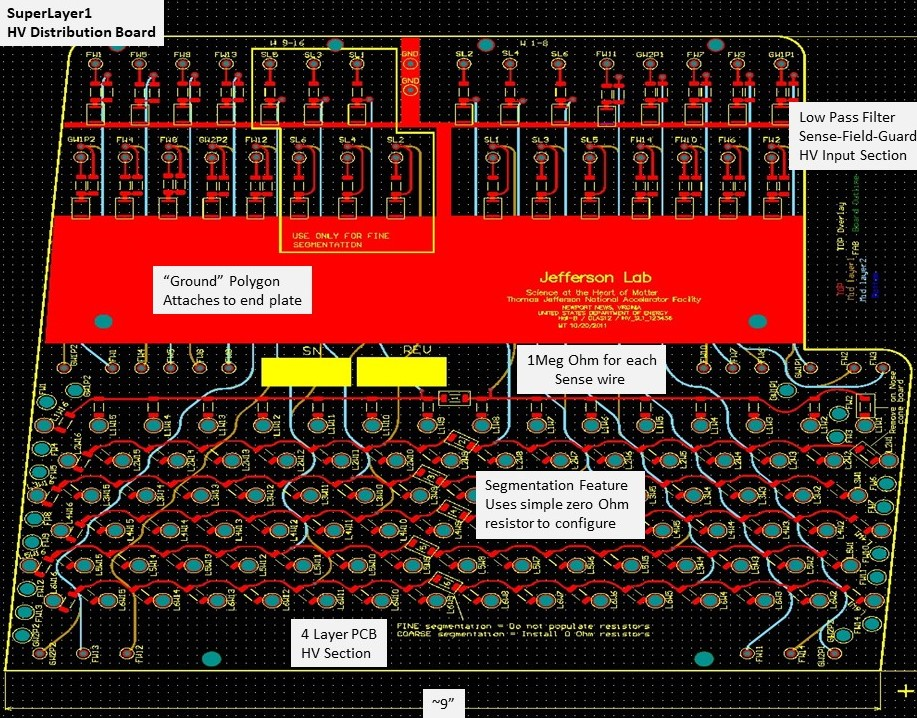
\includegraphics[width=0.7\textwidth,natwidth=610,natheight=642]{img/hvtb-layout.jpg}}}
\end{picture}
\caption{\small{Board layout drawing for the high-voltage translator boards.}}
\label{hvtb-layout}
\end{figure}
%%%%%%%%%%%%%%%%%%%%%%%%%%%%%%%%%%%%%%%%%%%%%%%%%%%%%%%%%%%%%%%%

The signal side of each chamber was tiled with 14 multi-layered printed circuit 
boards, (STB).  These boards were built in a 96-channel format that
requires seven circuit boards for each superlayer (672 signals). The boards capacitively
decoupled high-voltage from the signals, and then routed 
the signals to the SIP transimpedance preamplifiers 
mounted on the boards.  The amplified differential signals are then sent 
via 20-m long twisted-pair lines to the main CLAS12 readout electronics.

The connections between the sense-wire crimp pins and the plated-through holes 
of the STB boards were made using short conductive-elastomer tubes. This material 
consists of silver-plated and/or nickel-plated glass spheres embedded in a 
silicon-rubber matrix. These tubes pass through the plated-through hole and 
over the end of the crimp pins, making the electrical contract between the 
wire and the circuit board.  A small plastic cap inserted into the end of the 
tube ensures good contact with the circuit board.  This approach has the 
advantages of reducing the space needed for connections, preventing crimp pins 
from being pulled from the feedthroughs when disconnecting the boards from the 
wires, and reducing the cost compared to metal connectors.  This detail is 
shown in Fig.~\ref{wire-to-amplifier}.

%%%%%%%%%%%%%%%%%%%%%%%%%%%%%%%%%%%%%%%%%%%%%%%%%%%%%%%%%%%%%%%
\begin{figure}[htbp]
\vspace{8.5cm}
\begin{picture}(50,50)
\put(30,5)
{\hbox{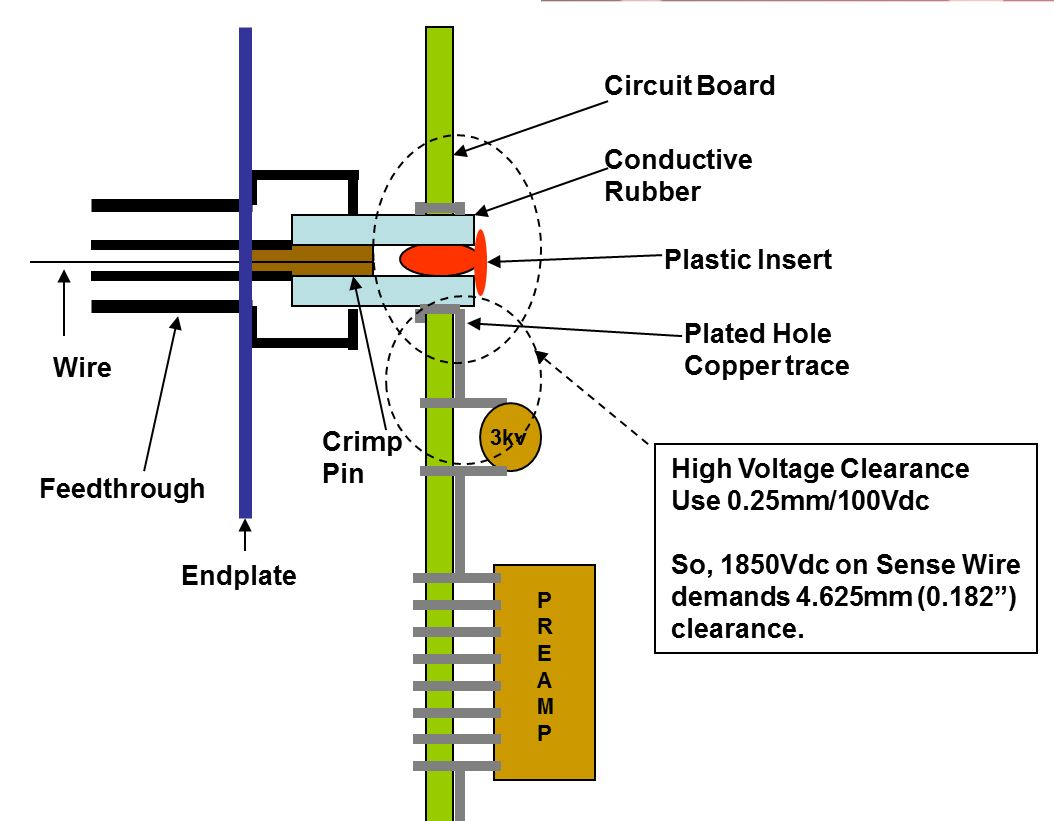
\includegraphics[width=0.7\textwidth,natwidth=610,natheight=642]{img/wire-to-amplifier.jpg}}}
\end{picture}
\caption{\small{ An assembly drawing showing how the crimp pin was inserted
into the feedthrough and how the conductive elastomer tube fits over the 
crimp pin and inside the plated-through hole on the printed circuit board to 
make the electrical connection. Also shown is the signal path from the wire's
crimp pin to the preamplifier.}}
\label{wire-to-amplifier}
\end{figure}
%%%%%%%%%%%%%%%%%%%%%%%%%%%%%%%%%%%%%%%%%%%%%%%%%%%%%%%%%%%%%%%%

Fig.~\ref{stb-layout} shows the layout of an STB board,
including the trace routings from the capacitively-coupled
wire signal to the SIP and the
placement of the SIPs into groups of 16 with the SIP outputs being
routed to the 16-pin signal connectors.  Also shown are the low-voltage
power traces with individual fuses for each group of 16 wires.
The board shown is from a R1 chamber, which had the tightest wire packing.

%%%%%%%%%%%%%%%%%%%%%%%%%%%%%%%%%%%%%%%%%%%%%%%%%%%%%%%%%%%%%%%%
\begin{figure}[htbp]
\vspace{8cm}
\begin{picture}(50,50)
\put(100,5)
{\hbox{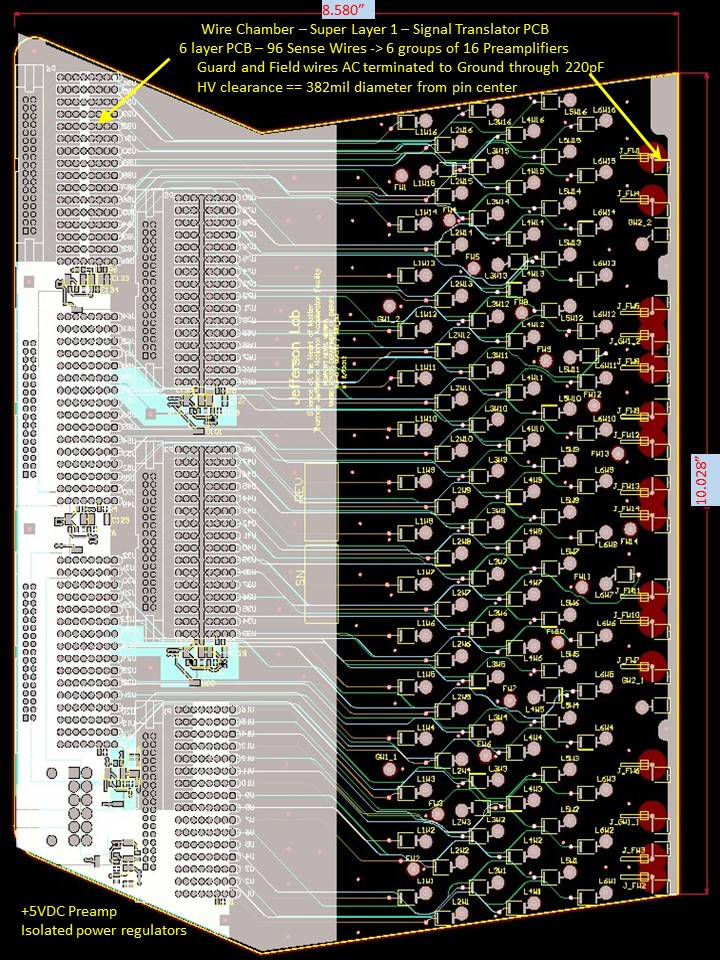
\includegraphics[width=0.1\textwidth,natwidth=610,natheight=642]{img/stb-layout.jpg}}}
\end{picture}
\caption{\small{Trace routing shown on one of the Region~1 STBs.}}
\label{stb-layout}
\end{figure}
%%%%%%%%%%%%%%%%%%%%%%%%%%%%%%%%%%%%%%%%%%%%%%%%%%%%%%%%%%%%%%%%

\subsubsection{Single Inline Package Preamplifiers}

The heart of the STB board is an individually packaged
single in-line package (SIP) preamplifer that was modified
from the design of the previous CLAS detectors and 
included an epoxy resin encapsulation.  
The encapsulation of the components prevents 
component corrosion in a somewhat humid environment (relative
humidities as high as 60\%).
These ``CP01'' preamplifiers provide the gain, dynamic range, rise time, low 
noise, and low power needed for the performance requirements.  The CP01 is
a transimpedance amplifier with a gain of 2 mV/$\mu$A and a rise-time
of less than 10 ns.  Each SIP operates at 5 V and draws about 13 mA.   
Fig.~\ref{CP01-description} shows the design and specifications of the
CP01 preamplifier.  See Ref.~\cite{fjb92} for the original design of
this SIP preamplifier.

%%%%%%%%%%%%%%%%%%%%%%%%%%%%%%%%%%%%%%%%%%%%%%%%%%%%%%%%%%%%%%%%%
\begin{figure}[htbp]
\vspace{8cm}
\begin{picture}(50,50)
\put(40,5)
{\hbox{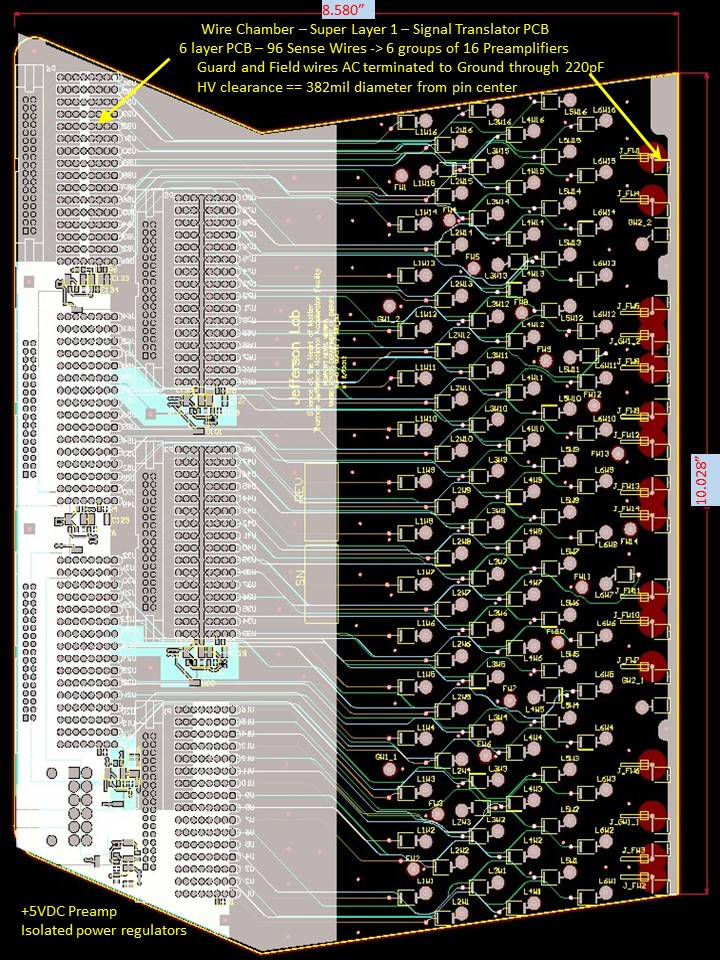
\includegraphics[width=0.7\textwidth,natwidth=610,natheight=64]{img/CP01-description.jpg}}}
\end{picture}
\caption{\small{The CP01 preamplifier design and specifications.}}
\label{CP01-description}
\end{figure}
%%%%%%%%%%%%%%%%%%%%%%%%%%%%%%%%%%%%%%%%%%%%%%%%%%%%%%%%%%%%%%%%%

Each group of 16 preamplifier output signals was routed to a 17-pair connector.
Sixteen of the pairs are used as differential signal paths that are routed from the STBs to the 
DCRBs over individual cables consisting of 16 twisted pairs. We chose
twisted-pair readout because of its immunity to electronic noise.
The cables are round-jacketed with a 
0.025-in pitch so that the overall cable dimension is smaller than the 
standard 17-pair cable.  

\subsection{Off-Chamber Amplification, Time Digitization, and Readout}

Our on-chamber preamplifiers send signals to the DCRBs, which provide another level of amplification, 
signal discrimination, adjustable threshold setting, time digitization, and readout. 



\subsubsection{Drift Chamber Readout Boards}

The DCRB is a 96-channel board that is a combination post-amplifier,
discriminator and time-to-digital converter (TDC); it also has a trigger
output path to provide track segment information for an online tracking trigger.
Fourteen such boards are housed in
a proprietary 9U, 160 mm depth, VXS form factor crate.
The whole system consisted of 18 such crates, one for each drift chamber.
See Ref.~\cite{daq-nim} for more details.

These DCRBs are based on FPGA technology, and in addition to
their primary function of amplification, discrimination, digitization,
and readout, they are used in a simple ``cluster-finding'' algorithm
to find track segment candidates with a latency of only hundreds
of nanoseconds.  For a more complete description of this please
see our companion article on the trigger, Ref.~\cite{trigger-nim}.

To perform its time digitization task, the DCRB utilizes on-board synchronization to
return the signal time relative to an input time signal from  a Trigger Distribution
Crate. Its design and architecture
allows it to achieve the following performance metrics:
\begin{itemize}
\item DCRB Performance Metrics
\begin{itemize}
\item Amplification: variable gain from X10 to X30 eliminates saturation
\item Time Digitization: accuracy better than 1 ns; exceeds DC specifications
\item Whole Crate Time Synchronization: through backplane; eliminates cables
\item Event Buffer Size: 500,000 signals
\item VME Transfer Rate: 200~MB/s
\item Maximum Trigger Rate: greater than 1~MHz
\item Dead-time: 32~ns
\item Scaler: 1 32 bit scaler per channel
\item Track Segment Finding: employs segment-hit dictionary in 32~ns bins
\item Track Segment Reporting: reports found segments to the next-level Track Finder
\end{itemize}
\end{itemize}

In addition to its primary functions of time digitization of DC signals and online
track-finding, the internal scaler functions allow the DCRB to be used in 
a stand-alone manner to efficiently monitor chamber operation during commissioning
and testing.

\subsection{Grounding Scheme}

We used a ``one-point'' grounding scheme.  The drift chambers themselves were insulated
from the torus magnet through use of an insulating portion of the link
mounting system.  The off-chamber DCRBs were likewise not grounded
to the chambers themselves though the use of non-grounded twisted-pair signals.
The low-voltage power supplies were floating, supplying a plus and minus line 
to the STBs.
The grounding point was at the high-voltage power supply crates.  This was accomplished
by the use of two ground wires for every high-voltage 34-wire multi-cable.


% -------------------------------------------------
% electronics
% -------------------------------------------------

\section{Drift Chamber Utilities: Gas, Low Voltage and High Voltage Systems}
\label{utilities}

\subsection{Gas System: Mixing, Monitoring and Pressure Control}

The chambers operate on a gas mixture consisting of 90\% argon and 10\% CO$_2$.
Using precision Mass-Flow Controllers (MFC), the gas is mixed and temporarily
stored in large-volume buffer tanks.  From these tanks it is delivered
to experimental Hall B.  

Argon is supplied via boil-off from a large, permanent dewar and CO2 is supplied 
via boil-off from several standard industry high-pressure Dewars.  Two identical mixing
systems are used to mix the gas to 90\% argon and 10\% CO$_2$ by mass using regulators and MKS G250 
mass flow controllers (MFC).  The mixed gas is then stored at ~100psig in four large-volume 
ASME pressure vessels, also called buffer tanks. This large volume smooths out 
any minor fluctuations in the argon/CO2 ratio. To control the gas ratio, the thermal 
conductivity of the gas ratio is continually measured using Panametrics Thermal 
Conductivity Units (TCUs) and then matched to the thermal conductivity of a mixed 
gas calibration standard. Individual MFC flows are adjusted as needed if the gas mixture
ratio changes. The mixed gas is supplied to the hall via two similar gas delivery systems, 
one for R3 and one for the combined flow through R1 and R2. 

MFCs and pressure regulators set the gas flow and pressure from the 
buffer tanks to the supply manifolds in the hall. In the hall, flow control for each 
individual sector is set using rotameters located at the supply manifolds. The gas flows 
into each detector at the nose and exits out of the back-plate and into the exhaust 
manifolds. Since the gas volumes of R1 + R2 = gas volume of R3, R1 and R2 exhaust 
through the same manifold and R3 exhausts through its own manifold. The exhaust manifolds 
are connected to pressure relief systems. 

The drift chambers use thin, aluminized Mylar windows with a large surface area.  
Any over-pressure event could cause the windows to burst. Likewise, an under-pressure 
event could cause damage to the wires inside.  Due to the potential of catastrophic 
damage to the detectors in the case of an over-pressure or under-pressure event, 
passive relief systems (bubblers) are installed on each exhaust manifold. In an 
over-pressure situation (i.e. high differential pressure between the exhaust manifold 
and atmosphere), the gas in the detector is vented out until the differential pressure 
falls to a safe level. In an under-pressure situation (i.e. low differential pressure 
between the exhaust manifold and atmosphere), air is sucked into the exhaust manifold 
until the differential pressure increases to a safe level. Each of these high-flow 
differential pressure relief systems consist of 3 parts:  An oil-filled over-pressure 
bubbler, an oil-filled under-pressure bubbler, and an empty oil trap, all filled
with high-purity mineral oil.  The oil trap is 
connected to the exhaust manifold while the over- and under-pressure bubblers are 
connected directly to the oil trap. This prevents contaminating the exhaust manifolds
with oil. Additionally, each of the 3 parts contains baffles to remove oil droplets 
from the gas passing through the unit. 

Fig.~\ref{dc-gas-system} is a schematic of the gas delivery system 
and a snapshot 
of the control panel for monitoring the state of the system.

%%%%%%%%% Figure : dc gas system %%%%%%%%%%%%%%%%%%%%%%%%%%%%%%%%%%%%%%%%%%%
\begin{figure}[htbp]
\vspace{6.7cm}
\begin{picture}(50,50)
\put(25,10)
{\hbox{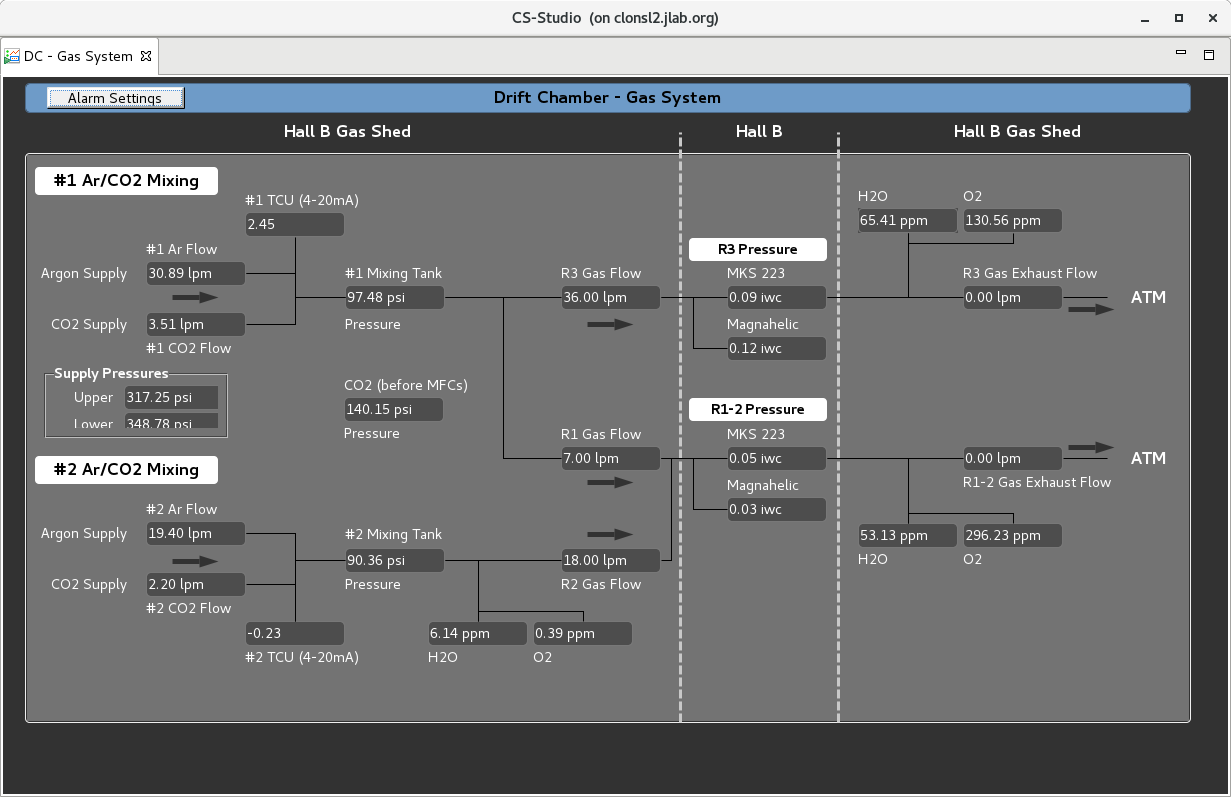
\includegraphics[width=0.6\textwidth,natwidth=610,natheight=642]{img/dc-gas-system.png}}}
\end{picture}
\caption{\small{A schematic of the drift chamber gas system showing key control and
monitoring points.}}
\label{dc-gas-system}
\end{figure}
%%%%%%%%%%%%%%%%%%%%%%%%%%%%%%%%%%%%%%%%%%%%%%%%%%%%%%%%%%%%%%%%%%
 
\subsection{Low Voltage System}
We reused the CLAS low voltage power supplies.  
These units are robust and manufactured by Hewlett Packard.  
The supplies are remotely programmable and monitored.  The on-chamber 
pre-amplifiers require 6 V and ~18 A per chamber
(a total of 1344 pre-amps per chamber).  

We isolated the low voltage from 
ground loops by using local voltage regulators on the pre-amplifier interface 
boards (STBs).  The segmentation of the low voltage distribution cables is 
based on 32 preamplifier channels per supply cable.  Each of the supply 
cables is fused for over-current 
protection based on the average current draw of 32 pre-amplifiers.  

We designed our low voltage system: supplies, fusing, cables, and control
system to be as robust and maintenance-free as possible.  To minimize
the damage to the tracking system in the event of a failure such as
a shorted pre-amplifier, we built in fine segmentation with only
32 preamplifier channels per supply cable. 
In the event of a short circuit that causes a fuse to blow,
a simple, external cable disconnect will reduce the size of the affected
area to 16 signal wires without the need to access the chambers.

Fig.~\ref{dc-lv-system} is a schematic of the low voltage
supply system and a snapshot 
of the control panel for monitoring the state of the system.

%%%%%%% Figure : dc low voltage system %%%%%%%%%%%%%%%%%%%%%%%%%%%%%%%%%%%%%%%%%%
\begin{figure}[htbp]
\vspace{8.5cm}
\begin{picture}(50,50)
\put(35,5)
{\hbox{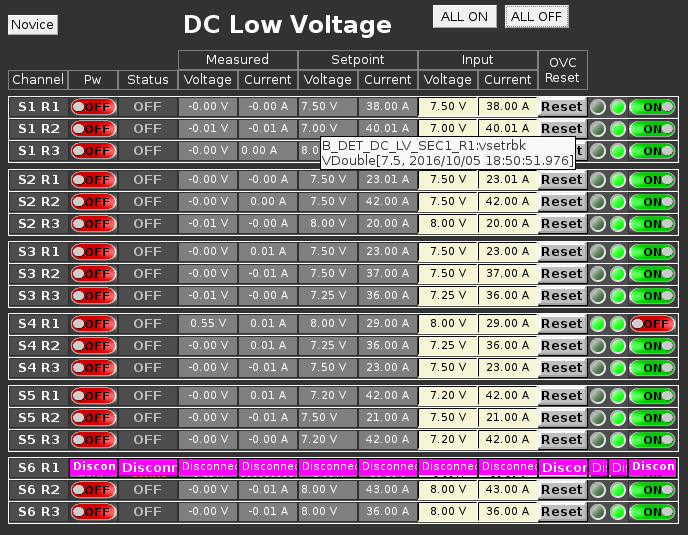
\includegraphics[width=0.9\textwidth,natwidth=610,natheight=642]{img/dc-lv-system.png}}}
\end{picture}
\caption{\small{A schematic of the low voltage control and monitoring scheme.}}
\label{dc-lv-system}
\end{figure}
%%%%%%%%%%%%%%%%%%%%%%%%%%%%%%%%%%%%%%%%%%%%%%%%%%%%%%%%%%%%%%%%%%%

\subsection{High Voltage System}

As in the case of the low-voltage system, we designed our high voltage system: 
supplies, distribution boxes, cables and control system to be as robust and 
maintenance-free as possible.  
We re-used our CAEN 
system 527 high voltage supplies with somewhat finer segmentation than our 
previous system, consistent with our total channel count dropping from 34000 
to about 24000.
To minimize the damage to the tracking system in the event of a failure such as
a broken wire, we built in very fine segmentation.
Each individual high-voltage channel powers a variable-sized group of 
wires: a 48-wire group for wires in the small-angle region, a 96-wire group
in the middle-angle region and a 192-wire group at large angles.

In the event of a failure (e.g. a broken wire) which results in a trip
of a single HV channel, we can further reduce the size of the affected
area from the whole group (48, 96 or 192 wires) to a smaller grouping
of 48 wires by an external cable disconnect without the need to 
physically access the chambers themselves.

The high-voltage supply and distribution system consists of the following:
\begin{itemize}
\item a crate-based high voltage power supply with 36 independent
high voltage channels for each drift chamber (1344 signal wires each).
Of these 36 channels, 16 supply positive high voltage to the sense
wires, 16 supply negative voltage to the field wires, and 4 supply
positive voltage to the guard wires
\item a series of two distribution boxes that distribute the high
voltage from the supply channels to variable-sized groups
of wires, with the group size being 8 wires (for small angle wires)
to 16 (intermediate angles) to 32 (large angles). 
\item  on-chamber printed circuit boards that distribute high voltage
to all of the wires; these are the HVTB's
\end{itemize}



Fig.~\ref{dc-hv-system} is a schematic of the high voltage
supply system and a snapshot 
of the control panel for monitoring the state of the system.
There are 648 individual remote-controlled high voltage channels
shown.  In this particular snapshot, two channels are colored
red (or darker) to indicate a high-voltage trip for the sense
and field wires for sector 2, R2, superlayer 1, wires 32-48.
The fact that the adjacent sense and field wire channels both
tripped indicate that there was an over-current condition for
this group of wires with current probably flowing from field to
sense wire; i.e. likely over-current in the chamber itself.
This happens occasionally when the beam is mis-steered, causing
higher than normal background radiation.

%%%%%%%%% Figure : dc high voltage system %%%%%%%%%%%%%%%%%%%%%%%%%%%%%%%%%%%%%%
\begin{figure}[hbtp]
\vspace{9cm}
\begin{picture}(50,50)
\put(5,5)
{\hbox{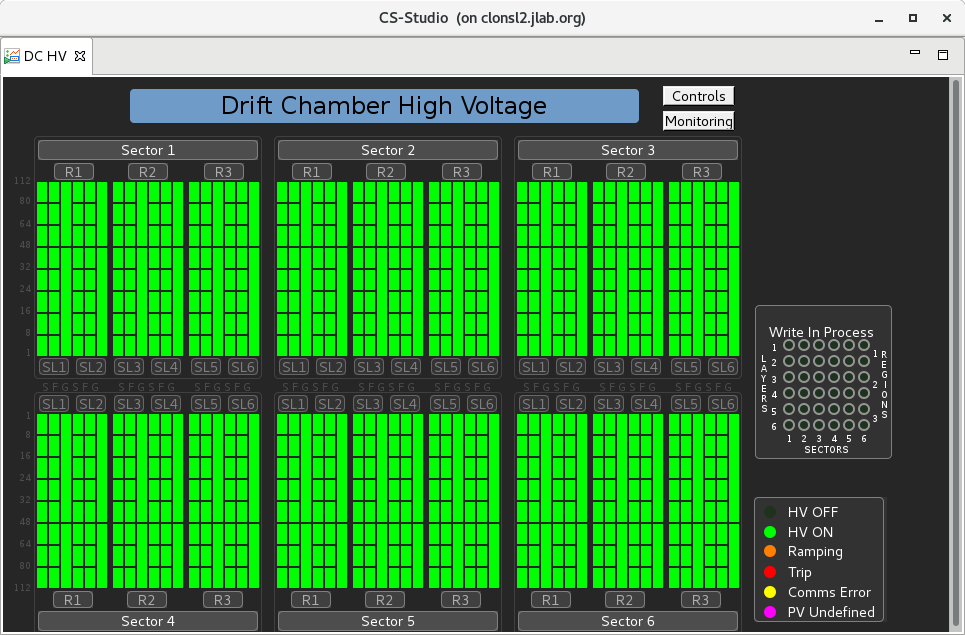
\includegraphics[width=0.8\textwidth,natwidth=610,natheight=642]{img/dc-hv-system.png}}}
\end{picture}
\caption{\small{A schematic of the high voltage control and monitoring scheme, showing
the 648 remotely controlled channels.}}
\label{dc-hv-system}
\end{figure}
%%%%%%%%%%%%%%%%%%%%%%%%%%%%%%%%%%%%%%%%%%%%%%%%%%%%%%%%%%%%%%%%%%




% -------------------------------------------------
% gas, lv, hv systems
% -------------------------------------------------

\section{Commissioning}

In this section we describe our procedures to do the following:

\begin{enumerate}
\item install electronics boards and ``on-chamber'' cables
\item gradually bring the chambers to full operating voltage (``burn-in'') 
and to test for any other problems
\item install and survey the chambers
\item diagnose and fix any early failures, and
\item perform efficiency scans over a range of HV and discriminator settings
\end{enumerate}

\subsection{Electronics Installation and Turn-on}
After the chambers were strung and went through a mechanical quality
check to insure that all wires are intact and properly tensioned, we
installed the on-chamber electronics boards.

There are two types of board: one is a High-Voltage Distribution Board (HVTB)
which brings RC-filtered high voltage to the wires.  Because there are three
types of wire: `sense', `field' and `guard' we supply three different voltages
to each board.  As discussed in the design section, we have a mixed high
voltage system: the sense (or anode) wires are operated at positive voltage,
typically about 2000 Volts; the field (or cathode) wires are operated at
about -1000 V and the guard wires at about +700 V.  This creates an
electric field which converges radially onto the sense wire with surface
field values of about 200 kV/cm.  Similarly each field wire has an
electric field directed radially outward from the surface with a strength
of about 50 kV/cm.  The surface field for the field wires is weaker 
because there are twice as many field wires as sense wires and their
diameter is larger (80 microns compared to 30).  The guard wires
close out the structure and their voltage is chosen to approximate an
infinite grid of wires; thus every sense and field wire in a superlayer
has the same field configuration unless there is an irregularity (like
a missing, broken wire) nearby.

On the other side of the chamber are our Signal Translator Boards (STB) 
which support an individual Single Inline Package (SIP) transimpedance
pre-amplifier for each sense wire.  This pre-amplifier takes the
small current pulse (microAmps) and translates it into a voltage 
pulse with a transimpedance of 2 mV/microAmp.  The signals (typically
10's to 100's of mV and 10's to 100's of nanosecond duration) are
transmitted down twisted-pair conducting wire to our downstream
Drift Chamber Readout Boards (DCRB) which further amplifies and
discriminates the voltage pulse and then converts the leading edge
to a digital time signal.
See figures (STB, HVTB) in the electroncis section for more details.

After stringing was complete we did the following:
\begin{enumerate}
\item ``daisy-chained'' the field wire crimp pins so that a single
HV cable could power two rows of field wires (32 wires)
\item physically positioned the boards so that their plated through
holes aligned directly above the sense wire crimp pins, and attached
the boards to the chamber with screws, and
\item electrically connected each sense wire crimp pin to each
plated through hole using a conductive rubber 'sleeve' which fit
over the crimp pin and also contacted the plated through hole on
its outer radius.
\end{enumerate}

Now the chamber was ready for ``burn-in'' and ``pre-testing''.

\subsection{``Burn-in and Pre-testing''}
When drift chambers are first turned on, they typically draw fairly high
`dark' currents, even at low voltages.  The standard procedure is to
slowly raise the high voltage, wait for a certain time period during
which the current subsides and raise the voltage again, and so on.
For our chambers, the typical time period was an hour and the typical
voltage step was 75 V which is approximately the `doubling voltage' of
our chambers (the voltage step which increases the gain by a factor
of two).

\subsection{Installation and Survey}
- chambers attached by ball and socket joints to rods which are attached
on the other end by ball and socket to the toroidal magnet frame



\subsection{Determining the Operating Values of the Discriminator Thresholds and High Voltage Settings}

We set the discriminator levels in the DCRB's to reduce the accidental hit rate (with no beam) due to electronic
noise to be less than about 1\%.  Since the electronic noise was generally proportional to wire length, we had less
electronic noise on the smaller R1 chambers.  Using this criteria, we set the thresholds to 30, 45 and 45 mV, respectively,
for R1, R2 and R3.  
Once we set the discriminator thresholds, we performed a High Voltage efficiency scan.  We raised the high voltage in
steps of 75 Volts and analysed the data.  We set the operating value for the high voltage at the point at which
the layer efficiency equaled or exceeded 97\%.

We determined the layer efficiency using the `excluded layer' method.  In one superlayer (of six layers) we found track
segments by our usual fitting method, but ignoring the data from a pre-selected layer (layer 3, for example).  We then
projected the track segment through that layer and determined whether or not the indicated wire (or an adjacent one) had a good hit.
Fig.~\ref{effcy-vs-voltage} shows the `plateau curve' of efficiency plotted versus voltage for one typical chamber 
and superlayer.  The layer efficiency at the chosen operating high voltage poiont was between 97\% and 98\%.

%%%%%%%%%%%%%%%%%%%%%%%%%%%%%%%%%%%%%%%%%%%%%%%%%%%%%%%%%%%%%%%%%%%%%%%%%%%
\begin{figure}[htbp]
\vspace{5cm}
\begin{picture}(50,50)
\put(-10,10)
{\hbox{\includegraphics[width=0.35\textwidth,natwidth=610,natheight=642]{img/trace-routing-schematic.jpg}}}
\end{picture}
\caption{\small{Layer efficiency plotted versus high voltage for a typical superlayer.}}
\label{effcy-vs-voltage}
\end{figure}
%%%%%%%%%%%%%%%%%%%%%%%%%%%%%%%%%%%%%%%%%%%%%%%%%%%%%%%%%%%%%%%%%%%%%%%%%%%


The single layer inefficiency is not uniform across the drift cell.  It is higher near the sense wire and also near the outer
edge of the cell.  A track passing close to a sense wire leave many ions in the cell, but the ion arrival times are stretched
out from near-zero to the maximum drift time, Tmax.  The result is that the pre-amplifier's output signal has a low voltage
amplitude but persists for a long time.  So, even though the collected charge is large the voltage put out by our trans-impedance
pre-amplifiers may not be large enough to exceed the voltage discriminator threshold of the DCRB,
For the case of tracks near the outer edge of the cell (so-called `corner-clippers') they simply leave a very small number
of ions in the cell and thus have a small signal.

In Fig.~\ref{effcy-vs-doca} we plot the layer efficiency as a function of the distance-of-closest-approach (DOCA) and
you can see the characteristic rise of the ineffiency near to and far from the sense wire.
%%%%%%%%%%%%%%%%%%%%%%%%%%%%%%%%%%%%%%%%%%%%%%%%%%%%%%%%%%%%%%%%%%%%%%%%%%%
\begin{figure}[htbp]
\vspace{5cm}
\begin{picture}(50,50)
\put(-10,10)
{\hbox{\includegraphics[width=0.35\textwidth,natwidth=610,natheight=642]{img/trace-routing-schematic.jpg}}}
\end{picture}
\caption{\small{Layer efficiency plotted versus DOCA.}}
\label{effcy-vs-doca}
\end{figure}
%%%%%%%%%%%%%%%%%%%%%%%%%%%%%%%%%%%%%%%%%%%%%%%%%%%%%%%%%%%%%%%%%%%%%%%%%%%


% -------------------------------------------------
% commissioning: ``burn-in and pre-testing'', installation and survey, lv, hv & gas hookup, signal connection
% turn-on, early failures and repair
% -------------------------------------------------

\section{Chamber Operation and Performance Monitoring}

\subsection{Choice of Gas}

The main requirements for the chamber gas were that it have reasonably low 
multiple scattering, allow for reasonable gas gains, have high drift velocities
in order to reduce the random background expected from M{\o}ller 
electrons and target-generated X-rays, and be inexpensive because of the 
large volume of the chambers. Also, safety considerations motivate the use of
a non-flammable gas mixture.  Additional concerns about small gas 
leaks and the proximity of many photomultiplier tubes argued against helium 
mixtures.  Ultimately a 90$\%$ argon - 10$\%$ CO$_2$ mixture was employed 
for several reasons: the gas has a fairly high saturated drift velocity 
($>$ 5~cm/$\mu$s), and it has an operating voltage plateau of several hundred 
volts before breakdown occurs.  The 90$\%$/10$\%$ mixture 
provides good efficiency and resolution, and reasonable collection times.

\subsection{Selecting the Proper Operating Voltage}

In this section we discuss our operating voltages and how it was determined.
First, we discuss how we divided the total voltage between our sense, field 
and guard wires in order to mimic a cell layout with an infinite number of
layers, achieving a situation in which all wires, regardless of layer, have
the same gain.  Then we discuss our choice of the total sense to field
wire difference in voltage; including the resulting gas gain and efficiency.


\subsubsection{Dividing the Total Voltage between Sense, Field and Guard Wires}
We ran our chambers with a mixed voltage scheme:
positive high voltage on the sense wires, negative voltage on the
field wires and positive voltage on the guard wires.
This mixed-voltage scheme has a couple of advantgages over a scheme in
which the field wires, for example, are held at ground potential:
\begin{itemize}
\item fewer field lines run from the sense wire to the endplate which
is grounded.  This reduces the likelihood of producing a ``Malter effect''
(Ref.~\cite{malter}) in which an accidental source of cathode emission
(due to an insulating contaminant on the endplate, for example) causes
a self-sustaining discharge
\item the sense to ground potential and the field to ground potentials 
are smaller; decreasing surface electric fields on the on-chamber
circuit boards
\end{itemize}

In addition, by carefully selecting the values of the sense, field and
guard wire voltages we can create potential distributions which mimic
an infinite grid of cells, where the gain on any wire is the same as
any other, regardless of whether is the first, last or middle layer.
See an early reference (\cite{mdm92}) for a discussion of this.

This optimum condition is reached when the sense voltage is twice the
field voltage (and opposite sign).  This is because we have twice as many
field wires as sense wires and all field lines which originate on a
field wire land on a sense wire.  

The guard wire voltage was then chosen so that the total charge on all wires is zero.  
If we have a nearby ground plane due to the metallized gas window, in general
there will be an induced surface charge which will affect the surface charge and
thus the gain of the nearby wire layers.  However, if the net charge on
all wires is zero, then there is no net flux of electric field through the
gas bag and thus the net charge on the gas bag is zero.  In this way all
of the wires have the same gain, regardless of layer.  

We used the drift chamber design program, GARFIELD, to determine the voltages
necessary to achieve the condition of net charge equal to zero.
The resulting ratio of voltages from Sense to Field to Guard wires is 1 : -1/2 : 5/14.

\subsection{Determining the Operating Values of the Discriminator Thresholds and High Voltage Settings}
\label{determine-operating-parameters}

We set the discriminator levels in the DCRB's to reduce the accidental hit rate (with no beam) due to electronic
noise to be less than about 1\%.  Since the electronic noise was generally proportional to wire length, we had less
electronic noise on the smaller R1 chambers.  Using this criteria, we set the thresholds to 30, 45 and 45 mV, respectively,
for R1, R2 and R3.  
Once we set the discriminator thresholds, we performed a High Voltage efficiency scan.  We raised the sense to
field wire potential
steps of 75 Volts and analysed the data.  We set the operating value for the high voltage at the point at which
the layer efficiency (the probability that a track passing through a layer will fire at least one wire) equaled or exceeded 97\%.

We determined the layer efficiency using the `excluded layer' method.  In one superlayer (of six layers) we found track
segments by our usual fitting method, but ignoring the data from a pre-selected layer (layer 3, for example).  We then
projected the track segment through that layer and determined whether or not the indicated wire (or an adjacent one) had a good hit.
Fig.~\ref{effcy-vs-voltage} shows the `plateau curve' of efficiency plotted versus voltage for one typical chamber 
and superlayer.  The layer efficiency at the chosen operating high voltage point was between 97\% and 98\%.

%%%%%%%%%%%%%%%%%%%%%%%%%%%%%%%%%%%%%%%%%%%%%%%%%%%%%%%%%%%%%%%%%%%%%%%%%%%
\begin{figure}[htbp]
\vspace{5cm}
\begin{picture}(50,50)
\put(-10,10)
{\hbox{\includegraphics[width=0.35\textwidth,natwidth=610,natheight=642]{img/trace-routing-schematic.jpg}}}
\end{picture}
\caption{\small{Layer efficiency plotted versus high voltage for a typical superlayer.}}
\label{effcy-vs-voltage}
\end{figure}
%%%%%%%%%%%%%%%%%%%%%%%%%%%%%%%%%%%%%%%%%%%%%%%%%%%%%%%%%%%%%%%%%%%%%%%%%%%



\subsubsection{Operating Voltage, Gas Gain and Layer Efficiency}
The gas gain varies exponentially with the total sense to field wire voltage
difference, with a doubling voltage of about 100, 110 or 120V respectively, for
R1, R2 and R3.  During our Fall 2019 run, we ran with sense - field wire voltage
differences of 2100, 2325 and 2475 V, respectively for R1, R2 and R3
We calculate that our total gas gain is approximately 2.7 X $10^4$, 3.7 X $10^4$, and 4.4 X $10^4$,  
respectively, for R1, R2 and R3.

\subsection{In-Run Performance Monitoring}
The CLAS12 detector records 10,000 - 20,000 events/sec during a typical experiment.
It is important that the experimenters who are running the data-taking be quickly
aware of any equipment malfunctions.

Our first level of monitoring comes from our hardware alarms; see our section on
Gas, LV and HV Utilities to see the control panels for our gas system and power
supplies.  Should these malfunction, an alarm is instantly shown on an alarm summary
screen with GUI-driven information on the lower-lying hardware monitoring screens.
An experimenter is thus able to detect an alarm and in most cases, reset the
alarming supply, within minutes.

Our second level of monitoring comes from on-line accumulating histograms.
Of these, the most important are our so-called ``Occupancy Plots'', which
are simply histograms of wire hits plotted versus wire number and wire layer (summed over
six superlayers in each sector).  Malfunctions show up
as depeleted areas on the plots.

Fig.~\ref{layer-vs-wire} shows a histogram of wire hits plotted as
a function of layer (1 - 36 on the vertical scale) versus wire number for each of the six
sectors.  A R1 chamber contains layers 1 - 12, a R2 chamber layers 13-24 and a 
R3 chamber layers 25 - 36. The horizontal axis shows the wire number in each layer (1 - 112).  
At a glance, one can inspect our ~ 24,000 wires and determine
that $>99\%$ of wires are functioning properly.  A few areas of inefficiency
are visible in the upper middle graph.  These correspond to
two areas in which the HV was disconnected to stop excessive current draw.

%%%%%%%%%%%%%%%%%%%%%%%%%%%%%%%%%%%%%%%%%%%%%%%%%%%%%%%%%%%%%%%%%%%%%%%%%%%
\begin{figure}[hbtp]
\vspace{10cm}
\begin{picture}(50,50)
\put(-10,10)
{\hbox{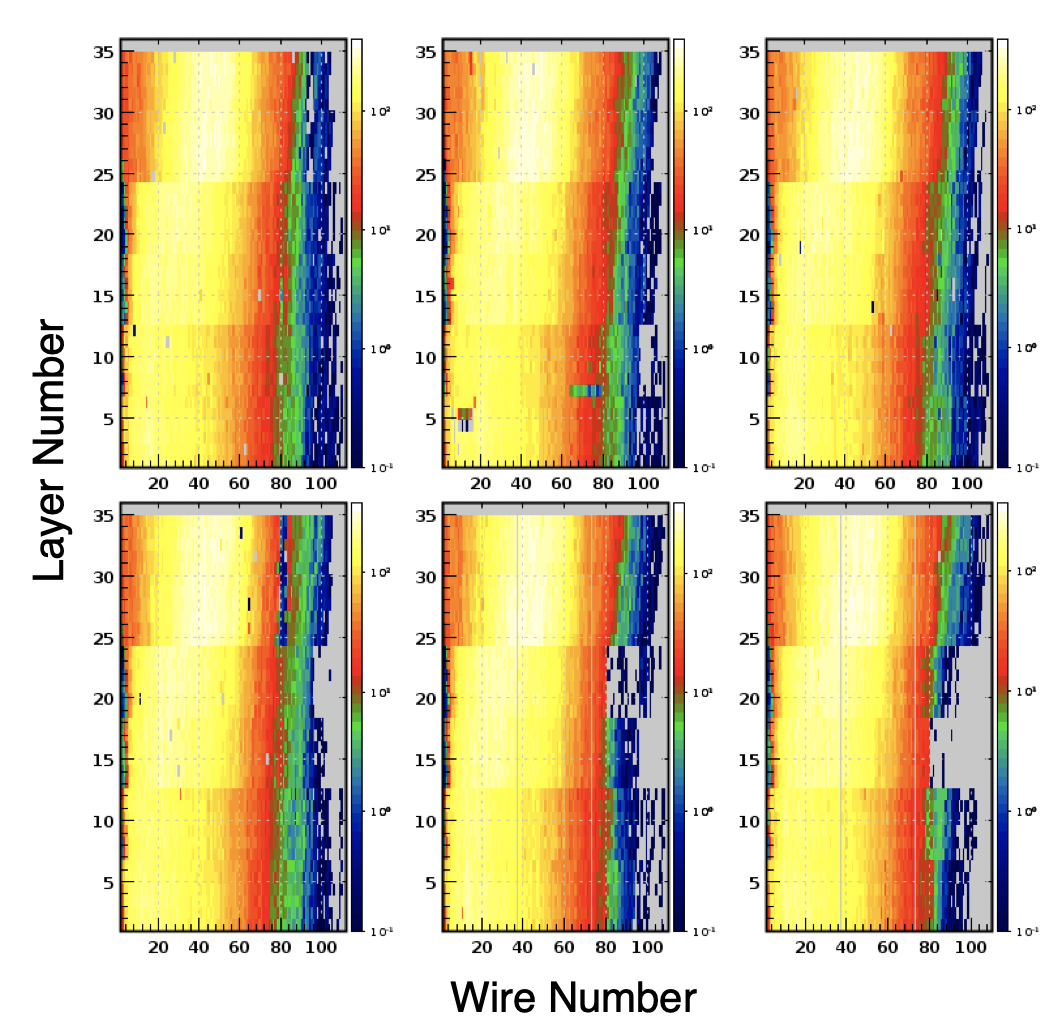
\includegraphics[width=1.\textwidth,natwidth=610,natheight=642]{img/layer-vs-wire.png}}}
\end{picture}
\caption{\small{An ``occupancy plot'' showing the number of wire hits accumulated over many events.
A few malfunctioning wire groups can be seen in the upper middle graph.}}
\label{layer-vs-wire}
\end{figure}
%%%%%%%%%%%%%%%%%%%%%%%%%%%%%%%%%%%%%%%%%%%%%%%%%%%%%%%%%%%%%%%%%%%%%%%%%%%



% -------------------------------------------------
%  operations and monitoring
% -------------------------------------------------

\section{Drift Chamber Calibration Procedures}
In this section, we discuss the calibration procedures to obtain the 
best possible spatial resolution for reconstructing the trajectory of
a forward-going charged particle.  We need to know three things to 
accurately reconstruct a trajectory: the location of the wires, the
distance of closest approach (DOCA) of the track to the wire and the
value of the magnetic field traversed.  These were determined by
\begin{itemize}
\item alignment procedures
\item time to distance calibration
\item magnetic field mapping and modelling
\end{itemize}.  

\subsection{Track Reconstruction Overview}

\hskip 0.15 in
The reconstruction of charged-particle tracks is performed in several stages.  In 
the first stage, individual tracks are fit only to hit-wire positions in a 
procedure known as ``hit-based'' tracking.  Hit-based tracking proceeds
in the following steps:
\begin{itemize}
\item in each superlayer, ``clusters'' of hits which are consistent with
being part of a track are identified
\item a ``noise rejection algorithm'' is then applied to the clusters, 
with one of the more efficient algorithms being the removal of the
interior hits from horizontal ``strings'' of hits along a layer.
\item the resulting trimmed clusters are then fit to a straight-line hypothesis,
and those hits with acceptable residuals are kept and identified collectively
as a ``track segment''.  This fit uses the wire position as the assumed hit
position and is called ``hit-based tracking''.
\item because the ``hits'' in a track segment are 2-dimensional objects (we
do not know their location along the wire direction) a track segment is not
a line but a plane.  Thus pairs of segments in neighboring superlayers within
one chamber (with superlayers of +/- $6^\circ$ stereo angle) represent the
intersection of two planes; that is a line.  This line's coordinates 
are evaluated midway between the two superlayers, and is a 6-dimensional
object (x,y,z and 3 angles) which we call a ``cross''.
\item in the first pattern-recognition step to find a track candidate,
the positions of 3 crosses (1 each in R1, R2 and R3) are fit to a
parabolic functional form to give us a ``track candidate''.
\item the track candidate is the initial ``state vector'' of our
Kalman filter tracking program 
\end{itemize} 

Due to the comparatively small size of the drift cells and the large 
number of wire layers, the track momenta can already be reconstructed 
at the ``hit-based'' level with a 
resolution of 3$\%$ to 5$\%$.  Additional information on these tracks, derived
from the {\v C}erenkov, time-of-flight, and electromagnetic calorimeter 
detectors, allows for determination of the identities and speeds of the 
charged particles.  In the second stage of the analysis, flight-time 
information of the particles from the target to the outer scintillators is 
used to correct the measured drift times.  A pre-determined table is then used
to convert the corrected drift times to drift distances (see section~\ref{tdistcal} 
for details of the function). These corrected 
track positions in each drift cell are input data to our Kalman filter
fit to determine the final track parameters.  This is colloquially referred
to as ``time-based tracking''.
The full track reconstruction procedure will be discussed in a separate paper.

\subsection{Alignment Procedures}
\label{align}

\hskip 0.15in
Each of the 18 drift chambers was 
surveyed with millimeter to sub-millimeter
accuracy, but we wanted an independent check of the chambers' positions and 
we needed to know the absolute position to better than 0.1 mm in order to 
achieve momentum resolutions on the order of 0.3\%.  For 
these reasons, the survey values for the chamber geometry were viewed only as 
a reasonable starting point to be refined by comparisons with data.

To adjust the chamber geometry parameters to improve the tracking resolution,
``straight-track'' data with the torus magnetic field off were analyzed.  
Tracks were found and fitted with our standard track reconstruction package.
For various bins in the angle of the track, we measured the shifts of the
track residual means as a function of layer number. 
Before correcting for mis-alignment in software, the data showed significant 
displacements of the means from zero, as large as 2 mm.  

Our procedure for aligment was straight-forward.  On a first pass through
the data we used misaligment parameters (shifts and rotations of individual
chambers) set to zero.  On subsequent passes, we deliberately misaligned
a particular chamber by a particular offset in position or angle and 
produced a second set of plots of residual mean vs. layer.  We ran 18 passes
through the data, adjusting all combinations of region (1, 2, 3) and
of offset type $\delta$x, $\delta$y, $\delta$z, $\theta$x, 
$\theta$y, $\theta$z, one at
a time.  The offsets in $x, y$ and $z$ were 2 mm, and the angular rotations
were 0.2 degrees.  These 2mm shifts and 0.2 degree rotations were
called ``unit distortions''.

We then subtracted the pass1 residual distribution from a pass``i'' distribution
to give a ``change of residual'' distribution caused by a given ``unit distortion''.
We then fit the observed residual distribution from the data to a weighted
sum of the 18 ``change of residual'' distributions.  In principle, we
could have had 18 free parameters, but in practice we had 12 free parameters:
 $\delta$ x, $\delta$ y, $\delta$ z, and $\theta$ y for each of the 3 chambers: R1, R2 and R3,
where $\theta y$ is a tilt of a chamber.  The yaw ($\theta x$) and roll ($\theta z$)
were not varied because they did not improve the fits.

Fig.~\ref{resids-vs-layer-before} plots the mean of the residuals of a straight-line
fit to the tracks versus layer (1 - 36 layers of the chambers), for each sector.
The misalignment is plainly visible as a noticeable shift of the residual means
from zero.  The bulk of the offsets occurs in shifts of groups of 12 layers which
corresponds to one physical chamber (a R1 chamber has layers 1-12, R2 from 13-24 and
R3 from 25-36).  
%%%%%%%%%%%%%%%%%%%%%%%%%%%%%%%%%%%%%%%%%%%%%%%%%%%%%%%%%%%%%%%%%%%%%%%%%%%
\begin{figure}[htbp]
\vspace{5cm}
\begin{picture}(50,50)
\put(-10,10)
{\hbox{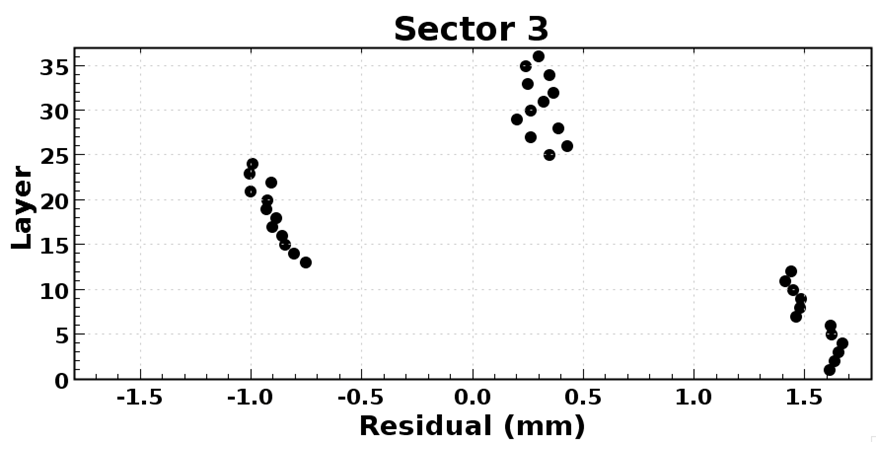
\includegraphics[width=1.\textwidth,natwidth=610,natheight=642]{img/resids-vs-layer-before.png}}}
\end{picture}
\caption{\small{A plot of the fit residual mean versus layer, before alignment.}}
\label{resids-vs-layer-before}
\end{figure}
%%%%%%%%%%%%%%%%%%%%%%%%%%%%%%%%%%%%%%%%%%%%%%%%%%%%%%%%%%%%%%%%%%%%%%%%%%%

Figure~\ref{resids-vs-layer-before} is the misalignment before our aligning procedure, while
Fig.~\ref{resids-vs-layer-after} shows the shifts of the means which remain after we have
aligned the chambers.
%%%%%%%%%%%%%%%%%%%%%%%%%%%%%%%%%%%%%%%%%%%%%%%%%%%%%%%%%%%%%%%%%%%%%%%%%%%
\begin{figure}[htbp]
\vspace{5cm}
\begin{picture}(50,50)
\put(-10,10)
{\hbox{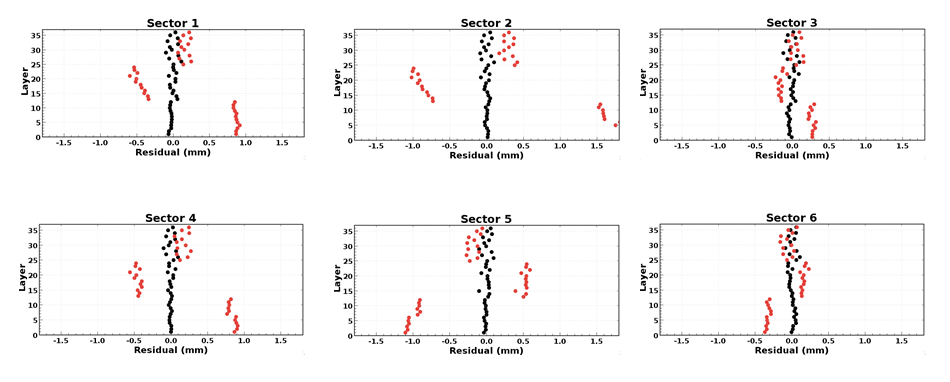
\includegraphics[width=1.\textwidth,natwidth=610,natheight=642]{img/resids-vs-layer-after.png}}}
\end{picture}
\caption{\small{A plot of the fit residual mean versus layer, after alignment.}}
\label{resids-vs-layer-after}
\end{figure}
%%%%%%%%%%%%%%%%%%%%%%%%%%%%%%%%%%%%%%%%%%%%%%%%%%%%%%%%%%%%%%%%%%%%%%%%%%%

The 
results of this procedure indicated that the best-fit position of the chambers 
along the three coordinate axes varied by up to several millimeters relative 
to the surveyed positions.  

\subsubsection{Geometrical Distortions}
The drift chamber internal geometry (placement of wires, etc.) was checked by detailed
surveys of the endplate, and of the endplates position with respect to the survey holes
located on the `nose' and `back' plates during construction of the full chamber assembly
and before stringing.
As discussed in the previous section, we surveyed the chambers into place on the
torus and also applied a `straight-track' analysis to fine-tune our knowledge
of the chambers geometrical location and orientation.

In addition to these alignment procedures which treat the chamber as a rigid, fixed
geometrical shape, we also measured and corrected two important chamber distortions:
\begin{itemize}
\item wire sagging due to gravity
\item bowing inward of the endplates in response to the collective wires' tension
\end{itemize}

The wire sag can be a large as 1mm for our 4 m long wires.  For this small
sag, it is sufficient to describe the shape of the sag as a parabola with
maximum deviation from a straight line occurring at the mid-plane of the chamber.
This correction to the hit position is thus applied at `event time' when 
the y-location of the hit has been determined.

The second type of geometrical distortion is due to the bowing of the endplates.
Because we wished to keep the endplates as thin as possible and because we did
not wish to obstruct the active area of the chamber volume with material, the
entire tension load was borne by the endplates which had a simple support at the
small `nose' plate and a fixed support at the 'back' plate.

We did extensive engineering analysis and also post-stringing survey to determine the
size and pattern of this bowing.  Because our endplate planes are not perpendicular to
the wires, when they bow they move the wire endpoints outward.  The amount varies
according to the chamber position because the weight of the endplates also plays a role,
but the bowing in the direction perpendicular to the wire could be as large as 1.5 mm.
This point of maximum deflection occurs about a fourth of the way between the `nose' and
`back' plates.  In Fig.~\ref{sketch-of-distortions} we show the engineering analysis
for a R2 enplate which agreed well with our direct surveys.

%%%%%%%%%%%%%%%%%%%%%%%%%%%%%%%%%%%%%%%%%%%%%%%%%%%%%%%%%%%%%%%%%%%%%%%%%%%
\begin{figure}[htbp]
\vspace{5cm}
\begin{picture}(50,50)
\put(-10,10)
{\hbox{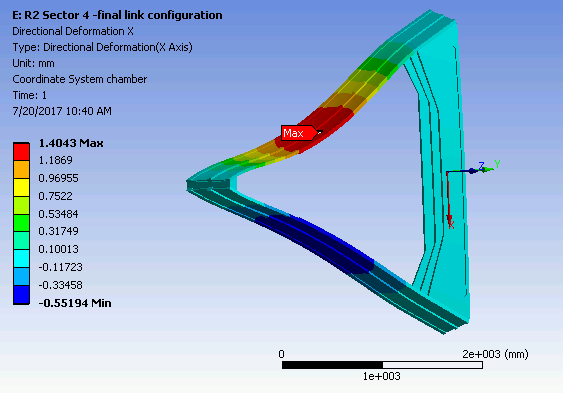
\includegraphics[width=1.\textwidth,natwidth=610,natheight=642]{img/sketch-of-distortions.png}}}
\end{picture}
\caption{\small{An engineering analysis showing the endplate bowing due to wire tension.}}
\label{sketch-of-distortions}
\end{figure}
%%%%%%%%%%%%%%%%%%%%%%%%%%%%%%%%%%%%%%%%%%%%%%%%%%%%%%%%%%%%%%%%%%%%%%%%%%%

\subsection{Time to Distance Calibration}
The drift chamber TDC's measure time.  This time is corrected for a number
of effects, and this corrected time is converted to a distance, DOCA, by 
a pre-calculated time to distance function.  In this subsection we 
explain the time corrections, the function used to calculate time as a 
function of DOCA and how we calibrate the parameters of this function.

\subsubsection{Time Corrections}
The drift time is the elapsed time between the time that the particle 
traversed the wire cell and the time that the released gas ions (electrons)
reached the sense wire.

The drift time is given by the following expression:
\begin{equation} 
\label{drift}
t_{drift} = t_{tdc} - t_{start} - t_{0} - t_{flight} - t_{prop} - t_{walk},
\end{equation}

\noindent
where $t_{TDC}$ is the raw time measured by the TDC, $t_{start}$ is the event start time, 
$t_0$ is the fixed-time (cable) delay for the wire, $t_{flight}$ is the 
flight time of the particle from the interaction vertex to the wire, $t_{prop}$ 
is the signal propagation time along the wire, and $t_{walk}$ is a time-walk 
correction made for short drift times due to different ionizations for slow 
and fast particles.  
With a trigger based on detecting an electron in the CLAS12 detector, the event start time is 
given by the time-of-flight counter time for the primary scattered electron 
corrected for the calculated flight time of this electron from the beam-target vertex.

As indicated in equation~\ref{drift}), the fixed-time delays (mainly fixed cable delays) 
for each wire must be known in order to determine the drift times.   To determine
this t$_0$ value, we produced a histogram of the following quantity for all hits
used on tracks:$ ( t_{tdc} - t_{start} - t_{flight} - t_{prop} - t_{walk} )$.
This produced a characteristic plot of a drift chamber signal on a flat
background from out-of-time tracks.  Our 24,192 drift chamber signals are carried
on individually made multi-conductor cables which each carred 16 signals.  We thus
produced and analysed 24,192/16 = 1512 histograms to determine that many values of
t$_0$. We occasionally re-do this analysis whenever we have a new trigger condition
or new configuration of readout boards.


\subsubsection{Time-to-Distance Functional Parameterization}
\label{tdistcal}

\hskip 0.15in
Each hit on a track is characterized by two variables, the measured drift 
time from the sense wire and the distance-of-closest-approach (DOCA) to the 
sense wire resulting from the track fit.  
A best fit to the dependence of DOCA on time defines the 
drift-velocity function of the drift cells. However, several factors 
complicate this analysis. For example, the DOCAs obtained from the fitted 
tracks are biased quantities since an initial estimate of the drift-velocity 
function is used in the track determination.  Moreover, the drift cells are 
not circular, as the analysis implicitly assumes, but are hexagonal, leading 
to angle-dependent corrections.   Also, the R2 chambers are in a 
region of high and spatially varying magnetic field.  Finally, the different 
ionization densities of the tracks from particles with different velocities 
leads to substantial time-walk corrections for tracks near the wire.  Each of 
these points is briefly discussed in this section.


%%%%%%%%%%%%%%%%%%%%%% Figure : Garfield Picture %%%%%%%%%%%%%%%%%%%%%%%%%%
\begin{figure}[htpb]
\vspace{4.5cm} 
\special{psfile=img/garfield.eps hscale=49 vscale=49 hoffset=-15 voffset=-130}
\caption{\small{Plot of electric-field lines and equal-time isochrone contours
(100 ns interval) for a 90$\%$ argon - 10$\%$ CO$_2$ gas mixture for (a) an R3
drift cell where two rays are drawn highlighting two different track entrance 
angles of $\alpha$ = 0$^{\circ}$ and 30$^{\circ}$, and (b) an R2 cell that 
was assumed to be located within a uniform 1~T magnetic field along the z 
direction.}}
\label{garfield-isochrones}
\end{figure}
%%%%%%%%%%%%%%%%%%%%%%%%%%%%%%%%%%%%%%%%%%%%%%%%%%%%%%%%%%%%%%%%%%%%%%%%%%%

Fig.~\ref{garfield-isochrones} shows the isochrone contours and electric-field lines for 
a representative R3 and R2 cell.  Note that the contours are circular close 
to the wire but become hexagonal near the outer boundaries of the cell.  This 
illustrates the necessity of knowing the entry angle of the track in order to 
determine the drift distance to the sense wire from the measured drift time.

\subsubsection{Function Parameterization}
\label{funcpar} 

In the CLAS detector, the drift distance was parameterized and fit as a function
of drift time.~\cite{mdm95}.
For CLAS12, we have instead chosen to parameterize the time as a function of
distance.  This is a more natural description of the drift chamber signal
for several reasons:
\begin{itemize}
\item the maximum drift distance is given by geometry (the distance from
a sense wire to the nearest field wire) and so it is fixed
\item the drift velocity is a function of electric field strength, so the
point of minimum field is the point of minimum velocity (and thus the inflection point on the T vs X curve). 
This inflection point of the curve occurs at a
definite value of distance within the cell and not at a definite value of time.
\item the time walk due to finite ionization is
naturally parameterized as a function of distance and not as a function of time.
\item two of the major time corrections (time walk which is a function of the
particle $\beta$ and a time correction for wires in a magnetic field, $B$ which
scales like $B^2$) can simply be added to the nominal functional form.
\end{itemize}

A {\bf single functional form} is used to fill two tables: one of time indexed by discrete
values of distance for use in the simulation by GEMC and one of 
distance indexed by time for use by the track reconstruction code.


\subsubsection{Choice of Mathematical Form for the Distance to Time Function}
We use a 4th order polynomial to model the distance to time relationship.

\begin{equation}
t(x) =  a x^4 + b x^3 + c x^2 + d x,
\end{equation}


By the use of simple calculus we convert the parameters a, b, c and d to equivalent parameters which have
a physically intuitive meaning.

\subsubsection{Physical Constraints on the Drift Velocity Function}

Inspection of  Fig.~\ref{garfield}a reveals that for tracks near the outer
edge of the cell, the first arriving ions follow the electric-field line from 
the field wire to the sense wire, independent of track entrance angle.  The
corresponding drift time is referred to as $t_{max}$ and occurs when DOCA is at its maximum value.

A second constraint is that the velocity near the wire is the ``saturated drift
velocity'' for our gas mixture, 90$\%$ argon - 10$\%$ CO$_2$.  We call this parameter $V_0$.
A third constraint is imposed by the fact that there is a definite point in the
cell at which the electric field is a minimum.  This implies that this is the point
of minimum velocity and is thus an inflection point.  This occurs at a value
$r = (x/x_{max}) = 0.615$ and the drift velocity at this point is termed $V_{mid}$.

\subsubsection{Constraints on the Parameters for the Polynomial Form}
In this subsection, we present the algebra for the constraints on the parameters
(a, b, c and d) of the polynomial form.  Because there are four free parameters, we
have imposed four constraints.

Constraints on the function coefficients:
\begin{itemize}
\item  $t(x)$ must equal $t_{max}$ when $x = x_{max} $.
\item  the drift velocity near the sense wire ($x = 0$)
must equal the saturated value, $V_0$
\item the function has an inflection point (a
mininum in velocity) at the point in the cell with the lowest electric field
strength.  From the geometry of our cells, this occurs at a distance
of $ 0.615 \times x_{max}$.  Finally,
\item the velocity equals $V_{mid}$ at the inflection point.
\end{itemize}

To summarize, these are the four constraints on the distance to time functions:
\begin{enumerate}
\item $t(x = x_{max}) = t_{max}$
\item $dt / dx (x = 0) = 1 / V_0$
\item $d^2 t / dx^2 (\hat{x} = 0.615 ) = 0$   
\item $dt / dx (\hat{x} = 0.615 ) = 1/V_{mid}$  
\end{enumerate}

In this way we convert our original parameters, a, b, c and d to the physically meaningful
parameters $t_{max}, V_0, r, and V_{mid}$ where $r$ is the value 0.615 (the fractional distance
at which the inflection point occurs) which can in principle also be varied.


\subsubsection{Dependence of Distance to Time Function on Local Angle}
\noindent
The preceding was the derivation for the function of time as a function
of drift distance for tracks with a local angle, $\alpha = 30^0$.  
We now discuss the
functional dependence on varying local angle and on non-zero and varying
values of the B-field.

Please refer back to Fig.~\ref{garfield} which shows a 0 degree track and a 30 degree
track, both at maximum distance from the sense wire.  Note that they will produce
a signal hit with the same time, Tmax, even though their distance-of-closest-approach d
iffers by a factor
of $cos(30^{0})$.  If Dmax is the distance from sense to field wire (and the maximum
DOCA possible for a 30 deg. track), then Dmax times $\cos(30^\circ-\alpha)$ is the maximum
DOCA for a track with local angle, $\alpha$.  Call this distance, $Dmax_{\alpha}$.

\subsubsection{Local Angle Dependence of Polynomial Form}
We derived the function for time versus distance for a particular local angle, $\alpha$, by
assuming the same functional form as for $\alpha = 30$ but with a {\bf different coefficient, a}, which 
satisfies the constraint that  $F(dmax_{\alpha},\alpha)$ = $t_{max}$.

Using this constraint, we can solve for $a_{\alpha}$ in terms of the known coefficients $V_0, ~a, ~n$, and $m$,
yielding the following:
\begin{equation}
\label{aalphaequation}
a_{\alpha} = {{t_{max} - b ~dmax_{\alpha}^3 - c ~dmax_{\alpha}^2 - d ~dmax_{\alpha}}\over{dmax_{\alpha}^4}}
\end{equation}

Using this formula for $a_{\alpha}$ we can derive the time as a function of distance and local
angle, $\alpha$ as shown in Fig.~\ref{xvst}.  See, for instance, the upper-left sub-figure 
which shows the time as function of distance for 5 different angles between $0^{\circ}$ and 
$30^{\circ}$, equally spaced in $\cos \left(30^\circ-\alpha\right)$.  Note two things:
\begin{enumerate}
\item for each angle, $\alpha$, the time is $t_{max}$ at $dmax_{\alpha}$, and
\item the distances for a given time vary with angle, $\alpha$, as $\cos \left(30^\circ-\alpha\right)$.
\end{enumerate}

The general functional form for time as a function of distance and local angle, $\alpha$
is given by
\begin{equation}
\label{tfunctionofxandlocalangle}
t(x,\alpha) = a_{\alpha} x^4 + b x^3 + c x^2 + d x
\end{equation}




\subsubsection{Dependence of Distance to Time Function on Magnetic Field Strength}
Since the R2 chambers are located within the field region of the CLAS torus, the 
magnetic field affects the drift velocity as shown in 
Fig.~\ref{xvst}b.  In particular, the field rotates and shrinks the isochrones
as shown in Fig.~\ref{garfield}b.  These effects can be modeled by a 
modification to the effective entrance angle of the track and by an increase 
in the time at a particular DOCA.  Both of these corrections are assumed to depend only on the 
magnitude of the magnetic field, and not its direction, following a study 
described in Ref~\cite{MM-IEEE}.  

The rotation of the isochrones is parameterized as a shift in the effective
entrance angle.  
\begin{equation} 
\label{eq-bcorrn-to-ang}
\alpha_b = \alpha_0 + \alpha_c \cos^{-1}(1 - a B), 
\end{equation}

The correction term $\alpha_c$ is determined from a 
GARFIELD simulation to be:

\begin{equation} 
\label{eq-bang}
\alpha_c = \cos^{-1}(1 - a B), 
\end{equation}

\noindent
where $a$ is a constant equal to $0.02$ and $B$ is the magnetic field strength in Tesla and angular
units are degrees.

%%%%%%%%% Figure : TRKDOCA vs. Drift Time -- Angle and Field Dependence %%%%%%%%%%
\begin{figure}[htb]
\vspace{15.cm} 
\special{psfile=img/tvsx.eps hscale=80 vscale=80 hoffset=-20 voffset=-10}
\caption{\small{Scatterplot of the corrected drift time versus TRKDOCA for 
(upper-left) R1, showing curves for various local angles from 30$^{\circ}$
(righmost curve) to 0$^{\circ}$ (leftmost curve).  (Upper-right) for R2; 
additionally showing 3 bands for B-field magnitudes of 0, 1, 1.5 Tesla.
(Lower-left) for R3 with the inflection point identified.}}
\label{xvst}
\end{figure}
%%%%%%%%%%%%%%%%%%%%%%%%%%%%%%%%%%%%%%%%%%%%%%%%%%%%%%%%%%%%%%%%%%%%%%%%%%%%%%%


The maximum drift time used in the time-to-distance function was extracted 
directly from the data.  For R2 the maximum drift time was parameterized as:

\begin{equation} 
\label{eq-bmax}
t_{max}(B) = t_{max}(0) + b B^2,
\end{equation}

\noindent
where $b$ is a constant and $B$ is the magnetic field strength.

At any given local magnetic field point, the distance-to-time function 
includes an additional correction term $\delta t_B$ to describe 
the magnetic field dependence.  See this reference~\cite{qin96} for a related
parameterization of the change in the distance at a particular time due to a
B-field. 

\begin{equation}
\label{XTB}
t(\hat{x},\alpha,B) = t(\hat{x},\alpha-\alpha_c, B=0) +  \beta(\hat{x})*B^2.
\end{equation}

\noindent
In this expression, the first term is the time calculated assuming B=0, and the
second term is the time increase due to the B field.  For the R1 and R3 functions, no magnetic field 
dependence is included, as the chambers are located outside the torus 
cryostats in regions that are relatively field-free.


\section{Determining the Distance to Time Function Parameters}
We determine the experimental values of the function parameters by fitting
a histogram of $TRKDOCA$ vs. time.

\subsubsection{Method of Calibrating the Time-to-Distance Function}
\label{tdistcal}

Each hit on a track is characterized by two parameters, the measured drift 
time from the sense wire and the distance-of-closest-approach (TRKDOCA) to the 
sense wire.  A best fit to the dependence of time on TRKDOCA determines the
values of the parameters of the drift-velocity function. 


\section{Using the Distance to Time Function in Reconstruction}
The track reconstruction program needs to know the expected distance as a function
of time.  However, as explained in the previous paragraph, we will have calibrated and fitted
the observed time as a function of distance.  So, we need to NUMERICALLY INVERT the t=f(x)
function in order to fill a table of X (real number) as a function of the time index (integer).

\subsubsection{Filling the Time to Distance and Distance to Time Tables}
We calibrate the distance to time function by fitting the drift time versus
TRKDOCA at a particular local angle, $\alpha$.  We write the independent parameters,
$V_0, ~V_{mid}$ and $T_{max}$ to the data-base.  At the beginning of a reconstruction program,
an {\bf inversion program} is run to numerical invert the function to produce a table
of distance indexed by time.


\subsubsection{How to Interpolate and Extrapolate in Local Angle}
Please refer back to Fig.~\ref{xvst} in order to understand the local-angle dependence
of distance versus time.  When the time is equal to $t_{max}$ the distance is equal to
the largest value for the local angle; that is, $dmax_{\alpha}$.  Also note that by
simple geometrical reasoning, $dmax_{\alpha} = dmax$  $cos(30-\alpha)$.
We assume that at times less than tmax and distances less than dmax, the calculated
distances still vary linearly as $cos(30-\alpha)$.  This angle dependence is built into
our functional form.

This means that we
\begin{itemize}
\item {\bf Fill} our time to distance tables for different local angles using the function, and
\item {\bf Interpolate} between time to distance tables for different local angles to obtain
the calculated distance at a particular local angle
\end{itemize}
For example if ``$X_0$'' is the distance (at a particular time) for a table filled for tracks with local angle of 0 degrees
and ``$X_{30}$'' is the corresponding quantity for a table of 30 degree tracks, then
\begin{equation} 
\label{eq-extrap30}
X(t,\alpha) = X_0 + (X_{30}-X_0) (cos(30-\alpha) - cos(30)) / (1. - cos(30))
\end{equation}

\subsection{Magnetic Field Model: A Comparison to Measurement}
In the Fall of 2016, we mapped the magnetic field of the torus magnet.
We documented the equipment and measurements in an article on the
construction of the torus (see Ref.~\cite{torus-ieee}) and in internal
documents (see Ref.~\cite{magmapping}).

We used three independent 1-dimensional Hall probes mounted in a precision-machined
Teflon holder.  The holder was a cylindrical solid which was pushed down a precision
Carbon fiber tube.  The probes were precisely spaced to be 5cm apart in the z-dimension,
with one oriented perpendicular to the z-axis, another perpendicular to the y-axis and
the third perpendicular to the x-axis.  In this way, we measured the x, y and z components
of the magnetic field at z-points separated by 5 cm along the axis of the toroid.

The Carbon fiber tube was positioned in x and y by precision machined ``endplates'' at the
upstream and downstream ends of the torus.  There were 24 precise hole locations on each
plate  (4 between each pair of torus coils).  We measured $B_x, ~B_y, ~B_z$ at 40 
locations in z at each of the 24 x, y locations, resulting in 2880 measurements.

By adjusting the six coils' shapes and locations, we were able to match our
magnetic model to the measurements to an accuracy of $0.5\%$.  Details of this
analysis will be available in a future publication, but in summary we
show in Fig.~$\ref{bmodel-bmeasured}$ the fractional difference between
the magnetic field from our model to that measured for the $40 X 6 = 240$ measurements
taken at 30 cm radius.  This is the region of the highest magnetic field (approx. 2 T)
and is most important for our low-angle, high-momentum tracks.  At the time of publication,
the average fractional difference was about 0.5\%.

%%%%%%%%%%%%%%%%%%%%%%%%%%%%%%%%%%%%%%%%%%%%%%%%%%%%%%%%%%%%%%%%%%%%%%%%%%%
\begin{figure}[htbp]
\vspace{5cm}
\begin{picture}(50,50)
\put(-10,10)
{\hbox{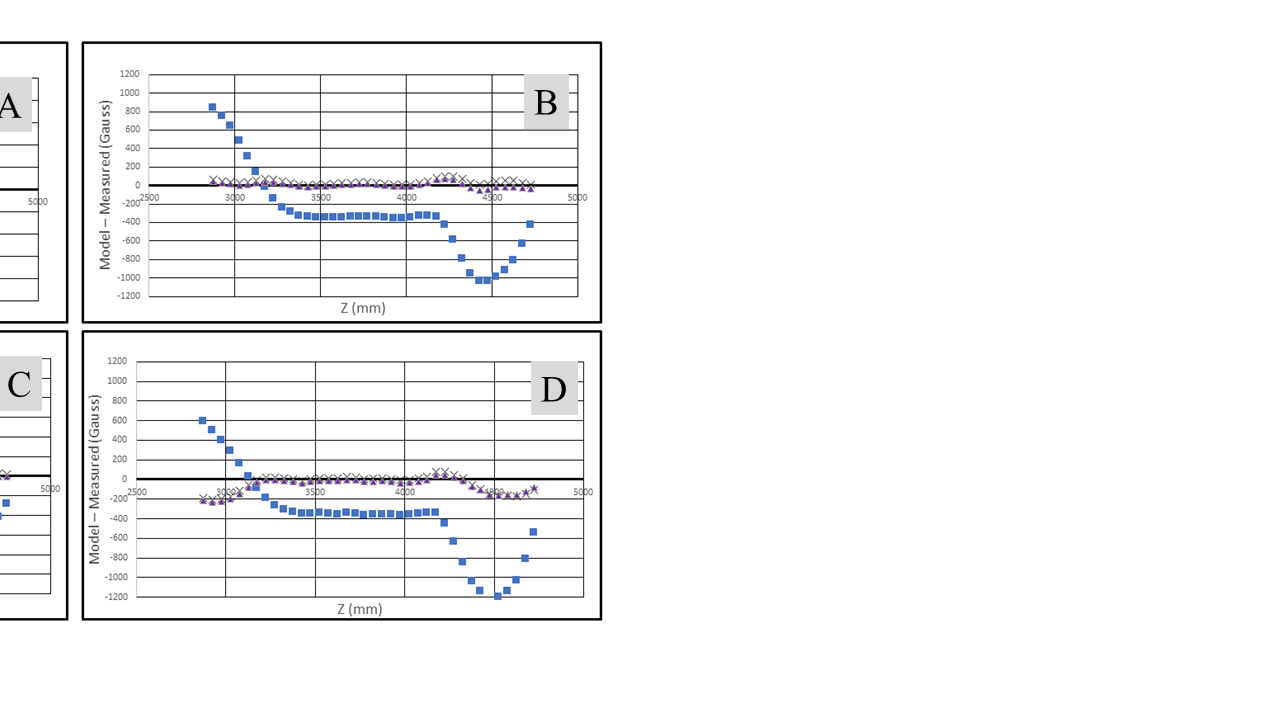
\includegraphics[width=1.\textwidth,natwidth=610,natheight=642]{img/bmodel-bmeasured.png}}}
\end{picture}
\caption{\small{A plot of (Bmodel - Bmeasured) / Bmodel versus z for the 240 measurement points
located at a radius of 30 cm and at the midplane between the 6 torus coils.}}
\label{bmodel-bmeasured}
\end{figure}
%%%%%%%%%%%%%%%%%%%%%%%%%%%%%%%%%%%%%%%%%%%%%%%%%%%%%%%%%%%%%%%%%%%%%%%%%%%



% -------------------------------------------------
%  tracking, calibration and simulation
% -------------------------------------------------

\section{Drift Chamber Tracking System Performance}

In this section, we describe the tracking system performance: the ability to operate at high luminosity,
the efficiency at reconstructing charged particle tracks, and the spatial resolution of such tracks.

\subsection{Operation at High Luminosity}

In order to satisfy the statistical requirements of the experimental program, an important design
goal for CLAS12 is the ability to make routine measurements with electron beam luminosities up to
10$^{35}$~cm$^{-2}$s$^{-1}$.  The luminosity limit in CLAS12 is 
set by the large flux of M{\o}ller electrons and low-energy photons 
produced from the targets by the multi-GeV incident electron beam.  This 
constraint is severe for the drift chambers since they are close to the 
target. 

Particularly for the R1 chambers, the large flux of particles limits the luminosity in several ways.
First, the chambers must be able to operate with an acceptably low trip rate.
Second, the accidental occupancy in the chambers should be on the order
of 5\% or less in order to keep the track-finding inefficiencies at a moderate 
level.  See the accompanying article on track reconstruction (\cite{recon-nim})
for a quantitative discussion of this effect.  Third, the effects of sustained high 
luminosities can be unfavorable for long chamber lifetimes.  Aging correlates 
directly with the currents generated in the chambers.
However, our choice of an argon-CO$_2$ gas mixture and strict control of
materials in contact with the gas should provide a long chamber lifetime.
For the previous CLAS chambers, we used the same gas mixture and ran at a
similar gain and similar currents, and the chambers operated for more than 10 years 
with no indication of aging.  We expect the present
chambers to perform well for at least 10 years.

\subsection{Tracking Inefficiency: Intrinsic, Malfunction-Related, and Background-Related}

The probability of not reconstructing a charged particle track due to a charged particle within our fiducial volume
is referred to as the ``tracking inefficiency''. The tracking inefficiency has three root causes:

\begin{enumerate}
\item intrinsic layer inefficiency: the failure to record
a hit for a track crossing a layer, when all wires and electronics
are operating properly;
\item malfunction-related inefficiency: loss of hits and sometimes
whole track segments because of equipment malfunctions;
\item background-related inefficiency: out-of-time background
can interfere with the segment-finding algorithms when a background-related
track segment lies ``on top'' of a real, in-time, segment.
\end{enumerate}

\subsubsection{Simulation of Inefficiencies}

In our generation and reconstruction of simulated events, we estimate the size of
the three types of inefficiency in the following manner:

\begin{enumerate}
\item simulation of intrinsic layer inefficiency: this is a random process
and, as such, it is handled at event generation time by our Geant4 Monte Carlo simulation
program GEMC~\cite{sim-nim}.  For each superlayer (1-6), we have defined a DOCA-dependent
layer inefficiency function, as determined from the data.  At hit-generation
time in GEMC a random number (between 0 and 1) is generated, and if it is
smaller than the layer inefficiency function, the hit is not digitized.
\item simulation of malfunction-related inefficiency: the GEMC Monte
Carlo hits are generated as if there are no malfunctions of the wires.
During the Monte Carlo reconstruction, however, a status table for each
hit wire is queried and if the wire is in the ``bad status'' list, that
hit is not used in the tracking. The malfunction-related inefficiency  is small.  
At this time, roughly 0.5\% of our wires are not operating properly.  
\item simulation of background-related inefficiency: rather than try
to simulate out-of-time background due to all physics processes, we merge
``random-trigger'' events with events from low-luminosity runs and compare the
efficiency of these merged events with that from un-merged low-luminosity events.
This ratio is considered to be a measure of the background-related inefficiency.
\end{enumerate}

We will not further discuss the malfunction-related inefficiency or
the background-related inefficiency further in this article.  See
our companion article on track reconstruction for more details~\cite{recon-nim}.
Here we present our results on measuring the intrinsic layer inefficiency.

\subsubsection{Intrinsic Layer Inefficiency}

The layer inefficiency is the probability that a
good hit is not recorded in a wire layer through which the track has passed, based on 
the evidence from all other layers in the superlayer.  This is called the 
``excluded-layer method''.  The layer inefficiency is a measure of the intrinsic drift 
cell inefficiency for the particular choice of gas mixture, high voltage set point, and 
discriminator level.  

The single layer inefficiency is not uniform across the drift cell.  It is slightly higher near the sense 
wire and substantially higher near the outer edge of the cell.  A track passing close to a sense wire 
leaves many ions in the cell, but the
ion arrival times are stretched out from near-zero to the maximum drift time $Tmax$.  The result is that
the preamplifier's output signal has a low voltage amplitude but persists for a long time.  So, even though
the collected charge is large, the output signal of our transimpedance preamplifiers may not be large
enough to exceed the voltage discriminator threshold of the DCRB. For the case of tracks near the outer
edge of the cell (so-called ``corner-clippers''), they leave a very small number of ions in the cell and
thus have a small signal.

Figure~\ref{dc-inefficiency-vs-doca} shows that the largest contribution to the drift cell
inefficiency is from tracks far from the wire.  These tracks may leave very few ions.  Even
tracks that are far from the wire but leave a substantial
number of ions can give rise to inefficiencies due to a large spread in ion arrival time.  
These tracks produce signals 
that have low pulse height and long duration, and thus may escape detection.
We fit this observed DOCA-dependent inefficiency to a functional form that is
used in our GEMC Monte Carlo hit digitization routine to randomly throw out
this percentage of hits.

%%%%%%%%%%%%%%%%%%%%%%%%%%%%%%%%%%%%%%%%%%%%%%%%%%%%%%%%%%%%%%%%%
\begin{figure}[htbp]
\vspace{7cm}
\begin{picture}(50,50)
\put(0,0)
{\hbox{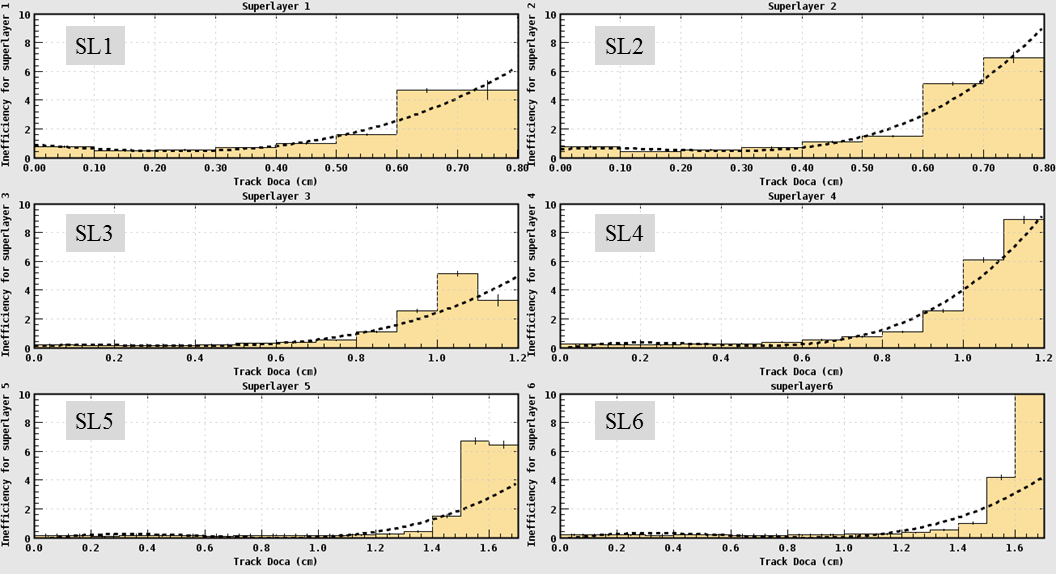
\includegraphics[width=0.8\textwidth,natwidth=610,natheight=642]{img/dc-inefficiency-vs-doca.png}}}
\end{picture}
\caption{\small{The observed layer inefficiency as a function of DOCA.  Hits from tracks
that pass close to or far from the sense wire have their signals spread out in time, and the resulting
voltage pulse from the preamplifiers may fail to cross the discriminator threshold, resulting
in a ``lost hit''.}}
\label{dc-inefficiency-vs-doca}
\end{figure}
%%%%%%%%%%%%%%%%%%%%%%%%%%%%%%%%%%%%%%%%%%%%%%%%%%%%%%%%%%%%%%%%%%%

The average layer efficiency of all wires (excluding the 0.5\% of malfunctioning wires)
is greater than 98\%.

\subsection{Drift Chamber Spatial Resolution}

The single-wire resolution is the RMS spread of the difference 
between the fit TRKDOCA of the track and the value of DOCA as calculated from the 
time of the hit.  The variance of this residual distribution 
is the quadratic sum of the single-wire resolution and the track position uncertainty.  
This variance over-estimates the single-wire resolution.
Since there are six layers per superlayer,
this amounts to a $10 - 15\%$ over-estimate.

Figure~\ref{resolution-vs-doca} shows the width of the track-hit residual distribution plotted vs.
TRKDOCA for each of the different chamber regions.  The single-wire resolution worsens near the 
wire and also at the outer edge of the cell.  This arises due to finite cluster sizes 
due to the Poisson distribution of ion-pair production along the path of the primary ion 
near the sense wire along with time-walk effects and the divergent nature of the electric
field lines near the field wire.  

%%%%%%%%%%%%%%%%%%%%%%%%%%%%%%%%%%%%%%%%%%%%%%%%%%%%%%%%%%%%%%%%%
\begin{figure}[hbtp]
\vspace{7.3cm}
\begin{picture}(50,50)
\put(50,-10)
{\hbox{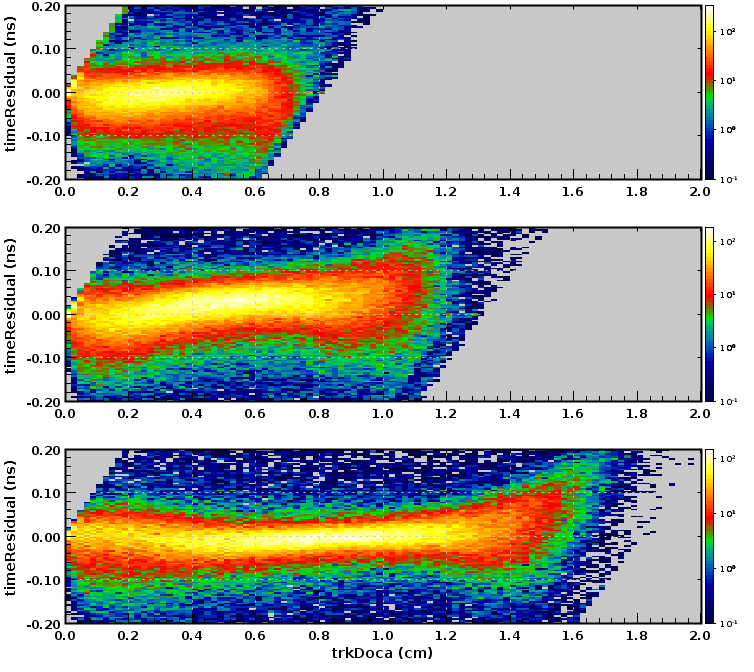
\includegraphics[width=0.85\textwidth,natwidth=610,natheight=642]{img/resolution-vs-doca.png}}}
\end{picture}
\caption{\small{The hit resolution plotted vs. TRKDOCA for R1, R2, and R3 (top, middle, bottom),
    respectively.}}
\label{resolution-vs-doca}
\end{figure}
%%%%%%%%%%%%%%%%%%%%%%%%%%%%%%%%%%%%%%%%%%%%%%%%%%%%%%%%%%%%%%%%%%%

A more quantitative look at the resolution is given in Fig.~\ref{gaussian-fit-to-resids}.
This is a plot of the residual distributions from each of the six superlayers in Sector 1; 
all sectors have similar results.
Because the resolution is narrow in the middle of the cell and widens considerably
for small and large values of DOCA (see Fig.~\ref{resolution-vs-doca}), we fit the
residual distribution to a double-Gaussian form. 
The average single-wire resolution in the middle 
portion of the cell is about 325, 395, and 310~$\mu$m for R1, R2, and R3, respectively,
with a whole cell resolution (RMS) is about 430, 540, and 515~$\mu$m for R1, R2, and R3, respectively.

%%%%%%%%%%%%%%%%%%%%%%%%%%%%%%%%%%%%%%%%%%%%%%%%%%%%%%%%%%%%%%%%%
\begin{figure}[htbp]
\vspace{7cm}
\begin{picture}(50,50)
\put(0,-5)
{\hbox{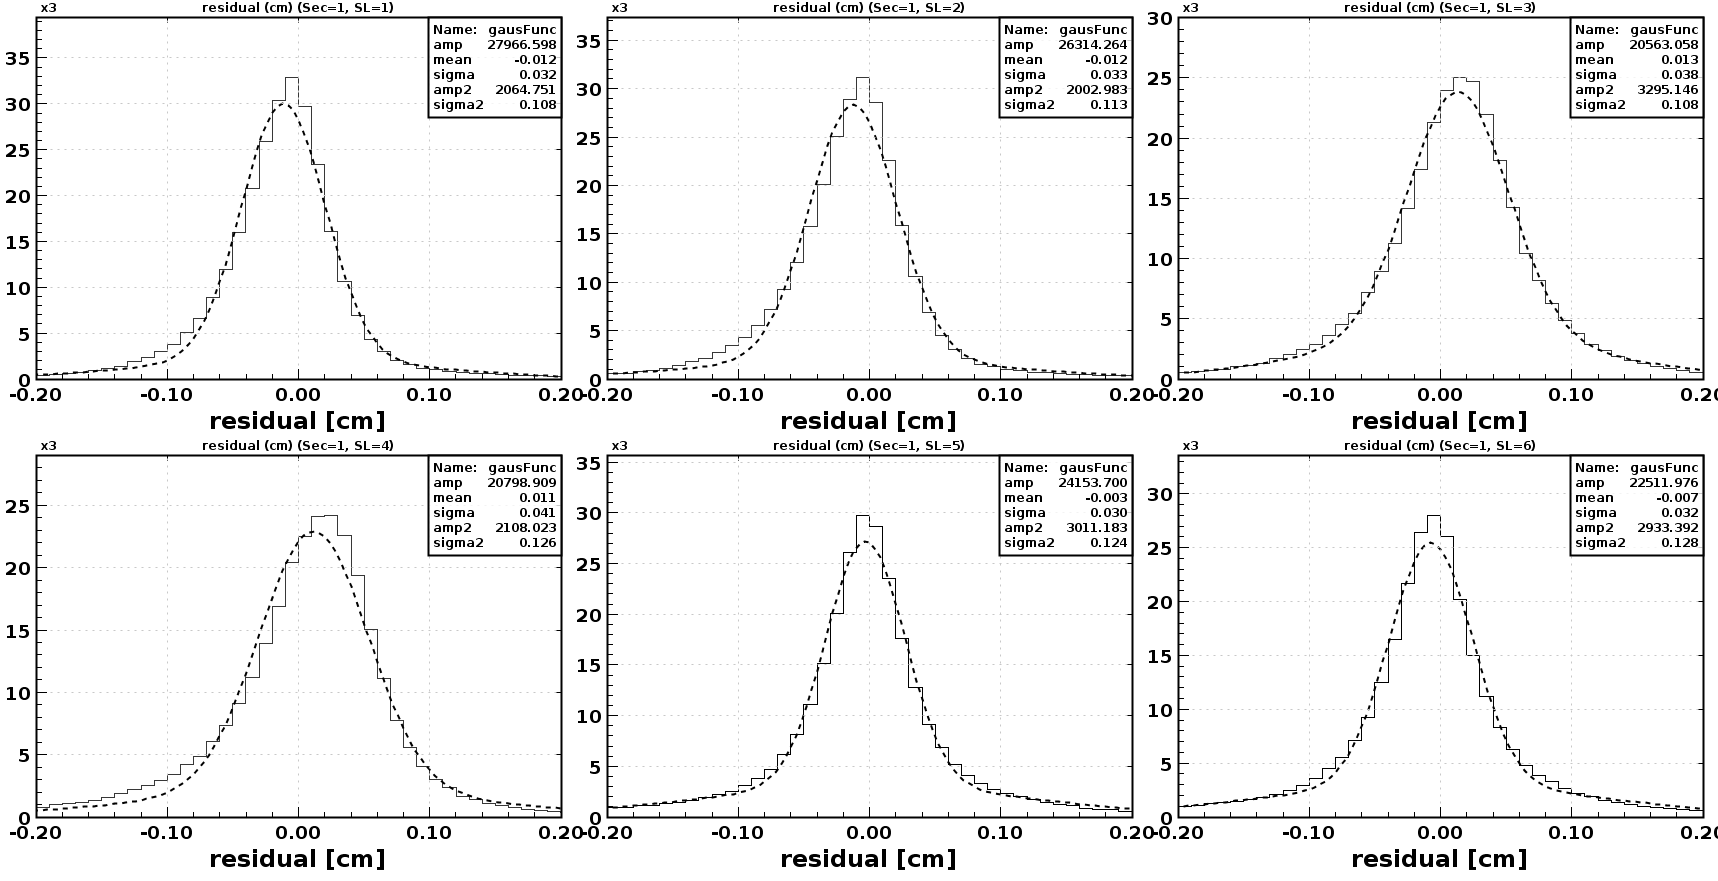
\includegraphics[width=.5\textwidth,natwidth=610,natheight=642]{img/gaussian-fit-to-resids.png}}}
\end{picture}
\caption{\small{A plot of the residual distributions for all 6 superlayers in Sector 1.  Over-plotted
is a double-Gaussian fit to the distribution.}}
\label{gaussian-fit-to-resids}
\end{figure}
%%%%%%%%%%%%%%%%%%%%%%%%%%%%%%%%%%%%%%%%%%%%%%%%%%%%%%%%%%%%%%%%%%%

\subsection{Summary of Design, Construction, and Operation}

The toroidal geometry of the CLAS12 spectrometer necessitated a particle-tracking 
system of unconventional design.  Design challenges and solutions include the following:

\noindent
- The necessity to conceal inactive areas of the drift chambers within the
shadow regions of the torus cryostat resulted in very thin endplates and low-profile
wire connection schemes and on-board preamplifiers.

\noindent
- The toroidal shape of the magnet and the desire to have measurements before, within, 
and after the high-field region, resulted in the design of a ``rod and ball'' mounting scheme
that minimizes dead areas and facilitates maintenance.

\noindent
- The fabrication of chambers that support large static wire tensions, but have thin 
endplates necessitated three endplate designs: aluminum stiffened with steel bars (R1),
Stesalit (an epoxy-fiberglass composite) stiffened with steel bars (R2), and thin stainless-steel 
plates filled with foam and reinforced
with carbon-fiber posts on the entrance side and a carbon-foam-carbon composite plate on the exit side (R3). 

\noindent
-The need for precise tracking in a system with non-saturated drift velocity 
(necessitated by the requirements of large drift distances, non-flammable gas mixtures, 
and low-gain operation) resulted in a semi-automated calibration and monitoring software 
package.

\subsection{Conclusions}

The CLAS12 drift chamber system has been in routine operation since spring, 2017. 
The system has reached its design goals of operating at high-luminosity
(1$\times$10$^{35}$~cm$^{-2}$s$^{-1}$) in a high-flux electromagnetic reaction
environment, with very good track reconstruction efficiency over a large range of angles and 
magnetic fields; see the article on track reconstruction~\cite{recon-nim}.  
The percentage of malfunctioning wires, due to high voltage problems, signal
connector issues, etc., is presently 0.5\%.
The single-wire efficiency is greater than 98\%.

Calibration efforts are ongoing, and at the time of this publication, the
single-wire resolution is about 500~$\mu$m averaged over all drift distances and
all 18 chambers.  The average single-wire resolution in the middle 
portion of the cell is about 325, 395, and310~$\mu$m for R1, R2, and R3, respectively.
\vskip 10 pt

{\large{\bf Acknowledgments}}

\vskip 10pt

The authors wish to thank the crews of wire stringers and technicians who 
participated during the chamber construction at Idaho State University,
Old Dominion University, and Jefferson Laboratory, as well as the support of 
the technicians involved with installation of the detectors into CLAS12. 
This material is based upon work supported by the U.S. Department of Energy,
Office of Science, Office of Nuclear Physics under contract DE-AC05-06OR23177,
as well as by DOE grants DE-FG02-87ER40315, DE-FG05-94ER40859,
DE-FG02-96ER40960, DE-FG02-96ER40980, and NSF grant NSF-PHY-9412479.






% -------------------------------------------------
%  track resolution and efficiency
% -------------------------------------------------

\begin{thebibliography}{99}

\bibitem{clas12-nim}
V.D. Burkert {\it et al.}, {\it ``The CLAS12 Spectrometer at Jefferson Laboratory''}, to be published in
Nucl. Inst. and Meth. A, (2020). (see this issue)

\bibitem{clasnim}
B.A. Mecking {\it et al.}, Nucl. Inst. and Methods A {\bf 503}, (2003) 513-553.

\bibitem{dcnim}
M.D. Mestayer {\it et al.}, Nucl. Inst. and Methods A {\bf 449}, (2000) 81-111.

\bibitem{kadyk}
J.A. Kadyk, Nucl. Inst. and Methods A {\bf 300}, 436 (1991).

\bibitem{nasa}
W. Campbell and J. Scialdone, ``Outgassing Data for Selecting Spacecraft Materials'', NASA internal
report RP-1124 Rev. 3 (1993).

\bibitem{cathode-emission}
S.B. Christo and M.D. Mestayer, ``Minimizing Cathode Emission in Drift Chambers'', CLAS-Note 92-016,
(1992). https://www.jlab.org/Hall-B/notes/clas\_notes92/92-016.pdf

\bibitem{patent}
U.S. Patent 8,863,568 ``Apparatus and procedure to characterize the surface quality 
of conductors by measuring the rate of cathode emission as a function of surface electric field 
strength'', Mac Mestayer, Steve Christo, Mark Taylor.

\bibitem{sbc}
S.B. Christo, ``Considerations for Crimping the CLAS Drift Chamber Wires'', CLAS-Note
89-021, (1989). \\ https://www.jlab.org/Hall-B/notes/clas\_notes89/note89-021.pdf

\bibitem{stesalit}
S. Bernreuther {\it et al.}, Nucl. Inst. and Methods A {\bf 367}, 96 (1995); W.L. Imhof {\it et al.},
Space Science Reviews {\bf 71}, 305 (1995).

\bibitem{stesalitaging}
R. Bouclier {\it et al.}, Nucl. Inst. and Methods A {\bf 350}, 464 (1994).

\bibitem{fjb92}
F.J. Barbosa, ``A Preamp for the CLAS DC'', CLAS-Note 92-003, (1992).
https://www.jlab.org/Hall-B/notes/clas\_notes92/note92-003.pdf

\bibitem{trigger-nim}
B. Raydo {\it et al.}, {\it ``The CLAS12 Trigger System''}, to be published in Nucl. Inst. and Meth. A, (2020).
(see this issue)

\bibitem{daq-nim}
S. Boyarinov {\it et al.}, {\it ``The CLAS12 Data Acquisition System''}, to be published in Nucl. Inst.
and Meth. A, (2020). (see this issue)

\bibitem{oxygen-contamination}
Y. Chiba {\it et al.}, Nucl. Inst. and Methods A {\bf 269}, 171 (1988).

\bibitem{malter}
L. Malter, Phys. Rev. 50, 48 - 58 (1936).

\bibitem{mdm92}
M.D. Mestayer, ``Choosing the Correct Combination of Sense, Field, and Guard Wire Voltage'', CLAS-Note 
92-005, (1992). https://www.jlab.org/Hall-B/notes/clas\_notes92/note92-005.pdf

\bibitem{GARFIELD}
GARFIELD has been developed at the University of Mainz by R. Veenhof and
revised by M. Guckes and K. Peters.  See HELIOS-Note 154, (1986).

\bibitem{ftof-nim}
D.S. Carman {\it et al.}, {\it ``The CLAS12 Forward Time-of-Flight System''}, to be published in Nucl. Inst.
and Meth. A, (2020). (see this issue)

\bibitem{mdm95}
M.D. Mestayer {\it et al.}, Nucl. Inst. and Methods A {\bf 367}, 316 (1995).

\bibitem{MM-IEEE}
M.D. Mestayer {\it et al.}, IEEE Transactions on Nuclear Science {\bf 39} No. 4, 690 (1992).

\bibitem{qin96}
L.M. Qin {\it et al.}, ``Performance of a Region II Drift Chamber Prototype and Region II Drift
Chamber Tracking'', CLAS-Note 96-018, (1996).
https://www.jlab.org/Hall-B/notes/clas\_notes96/note96-018.ps.gz

\bibitem{drift-velocity-results}
T. Zhao {\it et al.}, Nucl. Inst. and Methods A {\bf 340}, (1994) 485-490.


\bibitem{torus-ieee}
Probir K. Ghoshal {\it et al.}, IEEE Transaction on Applied Superconductivity, Vol. 29, No. 4, June 2019.

\bibitem{magmapping}
J. Newton {\it et al.} ``Measuring and Modelling the CLAS12 Torus Magnetic Field'', CLAS12-Note (to be written)

\bibitem{recon-nim}
V. Ziegler {\it et al.}, {\it ``CLAS12 Event Reconstruction''}, to be published in Nucl. Inst.
and Meth. A, (2020). (see this issue)

\bibitem{sim-nim}
M. Ungaro {\it et al.}, {\it ``The CLAS12 Geant4 Simulation''}, to be published in Nucl. Inst.
and Meth. A, (2020). (see this issue)

\end{thebibliography}



% -------------------------------------------------

\end{document}

